\chapter{Effect of Digital Elevation Model (DEM) Uncertainty on Geophysical Mass Flow via Identification of Strongly Coupled Subsystem}
\label{chap:dem}

\section{Introduction}
\label{introduction}

Eruptions from volcanic activities can spread along several kilometers causing catastrophic damages to lives and properties~\cite{volcano_world,volcano_us}. Volcanic eruptions are characterized by pyroclastic density currents (PDC), lahars, debris-avalanches and others resulting in a range of particles from small sand to boulders or mixtures of water and mud that travel up to several kilometers within a short range of time~\cite{boudon19931984,petrie1987terrain,takahashi2000mechanical, felix2004relation}. The hazard maps as a result encompasses a huge land area resulting in a large matrix required to represent the elevation profile~\cite{luhr1981colima,rueda2005erupciones,voight2013galeras,volcano_helens}. The need for high-resolution image study in such cases has always been a requirement. The recent 2010 Merapi Volcano in Indonesia generated PDC along a densely populated area causing huge death tolls and emergency evacuation~\cite{wiki_merapi}. The damage was further aided by debris-avalanche and lahars. The eruption exhibited fast and unequal depositions within a very short time range. Several reports, using high-resolution imageries investigated the impact of the volcanic eruption~\cite{charbonnier2013evaluation,jousset20122010, thouret114surono} for predicting catastrophes resulting from such an eruption in the future. %Even though there are abundant researches in this field, 
Geophysical mass flow resulting from the volcanoes pose a great threat due to uncertainty in topography of the rugged terrain, steep slopes, and uneven rock sizes. High resolution Digital Elevation Models (DEMs) capture small variations in a terrain profile that can that can be used for enabling accurate computational fluid dynamics (CFD) simulations to predict the flow of ground hugging flows such as PDCs or lava flows more accurately. Although, modern aerial photographies can enable capturing high-resolution images of a volcanic region, there still can be errors in DEMs~\cite{mitasova1996modelling}. Quantifying the effect of uncertainty in high-resolution DEMs on a volcanic flow is a computationally expensive problem. 
%The main focus of this work is to propagate the uncertainty in DEMs for geophysical mass flow simulation via Titan2D~\cite{patra2005parallel} by generating fewer realizations for the uncertain DEM profile. This lower order sampling is achieved by using a recently developed method of identification of Strongly Connected Subsystems (SCSs) in a dynamical system~\cite{Mukherjee_2017overlap}.


Uncertainty Quantification (UQ) in a geophysical mass flow problem refers to estimating a probabilistic hazard map (PHM) that can result from the flow of volcanic eruption provided by a CFD simulation. Such a detailed analysis showing the probabilistic extent of a PDC or lahar flow can benefit the neighboring area of a potential volcanic region. In the past, PHM has been generated by considering uncertainty in model parameters. Jibson and Herp~\cite{jibson2000method} has estimated the PHM of a seismic activity due to uncertainty in shear strength. Somerville \textit{et al.}~\cite{somerville1997modification} has studied rupture activities by exploring uncertainties in ground motion parameters. Uncertainty in input parameters for rhyolitic eruption such as plume height, eruption mass, grain size distribution, eruptive vent and others have also been investigated~\cite{bonadonna2005probabilistic}. 


Due to advances in digital of photography and advanced computing power, DEMs can be created for almost every location on earth. %accurately with a very high spatial resolution. 
However, small errors in elevation profile persist due to measurement error or due to interpolation methods used. Therefore, the DEMs are not completely accurate. 
DEM uncertainty modeling and and its effects in estimating PHMs has always been a challenge owing to the size of the problem. Characterizing the DEM error is a non-trivial problem, since it requires the estimation of spatial correlation over a large area. Specially, modeling the spatial error requires rigorous investigation. Although, stochastic modeling of a DEM is not a current aim, this work focuses on the error in DEMs that can lead to difference in PHM. DEM error propagation in slope and aspect by Monte Carlo simulation has been studied by Heuvelink \textit{et al.}~\cite{heuvelink1998error}. Similar studies has also been made by Oksanen~\cite{oksanen2005error,oksanen2006digital}. Weng~\cite{weng2002quantifying} quantified the error due to topographic map, measurement, and interpolation process separately and their overall contribution to total error-propagation. 


% Further to minimize computational time and avoiding the simulation of the actual physics-based model, surrogate models have also been developed to estimate hazard maps. 

% \begin{itemize}
% \item High-resolution landform classification using fuzzy k-means -- classification of land area into features
% \item CFD-DEM simulations and experimental validation of clustering phenomena and riser hydrodynamics -- clustering on the resultant flow
% \end{itemize}

% \begin{itemize}
% \item modeling DEM uncertainty~\cite{hebeler200914}
% \end{itemize}


The current chapter extends the SCS-based UQ idea to form a fourth order tensor graph adjacency for a large square matrix and eventually apply overlapping graph clustering technique on the matrix form of the adjacency. The clustering technique identifies subregion that can be used individually in parallel to simulate sample realizations while keeping the rest of the DEM at a nominal value. This process helps in creating a sampling space for the terrain profile of much lower order than given by traditional sampling methods. The flow simulation is then run on every realization of this sampling space using the Titan2D software. PHMs are generated based on the output of the simulation run on this sampling space. 

Figure~\ref{fig:scs_titan} shows the schematic of PHM generation using Titan2D on an actual volcanic region integrated with the SCS-based UQ methodology. Given a volcanic location (Figure~\ref{fig:scs_titan}(a)) and the uncertainty model of the DEM (Figure~\ref{fig:scs_titan}(b)), the state-space equation (Figure~\ref{fig:scs_titan}(c)) is used a graph-theoretic representation to model the inter-state coupling (Figure~\ref{fig:scs_titan}(d)). This graph is used to formulate an associated graph adjacency (Figure~\ref{fig:scs_titan}(e)) and corresponding SCSs (Figure~\ref{fig:scs_titan}(f)). This cluster structure is used to sample realization and simulate them via Titan2D (Figure~\ref{fig:scs_titan}(g)). The result of the simulations from each SCS is used to compute the PHM. 

\begin{figure}[H]
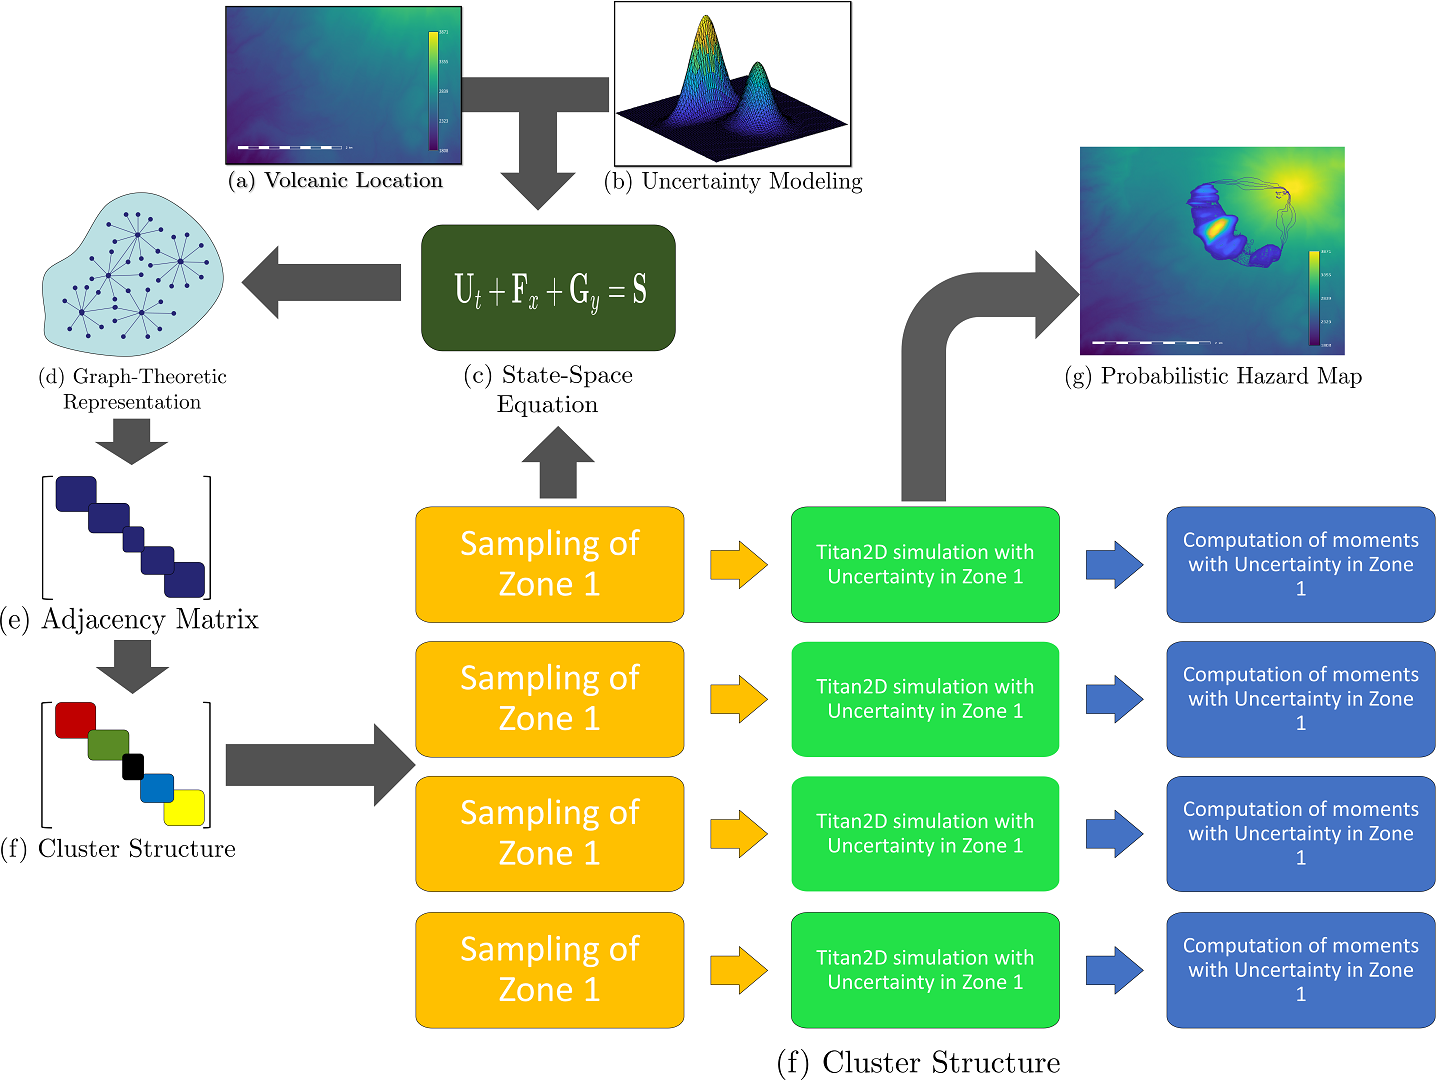
\includegraphics[width=\textwidth]{dem_figs/dem_framework}
\caption{Schematic of the SCS identification-based UQ to estimate PHM for geophysical mass flow using Titan2D}
\label{fig:scs_titan}
\end{figure}

\section{Governing Equations}
\label{governing}
The incompressible continuum geophysical mass flow equation is modeled as the conservative form of the shallow-water equations. The equation follows from the depth-averaged Savage-Hutter equation of flow of granular mass~\cite{savage1989motion}. The set of equations are derived in a coordinate system OXYZ parallel to the basal surface in terms of the depth-averaged components. The non-dimensional form of the equations are:

\begin{equation}
\label{main_eq}
\frac{\partial \textbf{U}}{\partial t} + \frac{\partial \textbf{F}}{\partial x} + \frac{\partial \textbf{G}}{\partial y} = \textbf{S}
\end{equation}

\noindent where, 

\begin{equation}
\label{defs}
\begin{array}{c}
\textbf{U} = \begin{bmatrix}
h \\ hv_x \\ hv_y
\end{bmatrix} \\
\textbf{F} = \begin{bmatrix}
hv_x \\ hv_x^2 + \frac{1}{2}k_{ap}g_x h^2  \\ h v_x v_y
\end{bmatrix} \\
\textbf{G} = \begin{bmatrix}
hv_y \\ hv_xv_y \\ hv_y^2 + \frac{1}{2}k_{ap}g_y h^2  
\end{bmatrix} \\
\textbf{S} = \begin{bmatrix}
0 \\
g_x h - h k_{ap} sgn \left( \frac{\partial v_y}{\partial x} \right) \partial_y \left( g_z h \right) \sin \phi_{int} - \frac{v_x}{ \sqrt{v_x^2 + v_y^2}} \left[ g_z h \left( 1+ \frac{v_x}{r_x g_z} \right) \right] \tan \phi_{bed} \\
g_y h - h k_{ap} sgn \left( \frac{\partial v_x}{\partial y} \right) \partial_x \left( g_z h \right) \sin \phi_{int} - \frac{v_y}{ \sqrt{v_x^2 + v_y^2}} \left[ g_z h \left( 1+ \frac{v_y}{r_y g_z} \right) \right] \tan \phi_{bed}
\end{bmatrix}
\end{array}
\end{equation}

\noindent The unknowns of the equation in $\textbf{U}$ are the pile height $h$ and the momentum components in $x-y$ directions. The dissipative source term comprises of the gravitational force and the dissipative internal and basal frictional forces in the $x$ and $y$ directions. A Coulomb-type friction term at the interface between the dry avalanche and the basal surface is considered for solving the mass-momentum set of equations. The internal friction of angle of the medium is $\phi_{int} = \tan^{-1} (\sigma_t /\sigma_n)$ and the angle of friction between the material and the basal surface is $\phi_{bed}$. The active/passive stress coefficient $k_{ap}$ is defined as,
\begin{equation}
k_{ap} = 2 \frac{1 +\pm \left[ 1 - \cos^2\phi_{int} \left( 1+ \tan^2\phi_{bed} \right) \right]^{1/2}}{\cos^2 \phi_{int}} - 1
\end{equation}

\noindent Here $\lbrace g_x, g_y, g_z \rbrace$ are the components of gravity in $x,y,z$ direction and $r_x, r_y$ are the radius of curvature of the basal surface. 

The governing equations in~\ref{main_eq} is solved using the simulation software TITAN2D~\cite{patra2005parallel,SHERIDAN200589}. The approximate Reimann problem for the system is solved by the software using finite volume method. The fluxes are computed as cell averages using the first-order Godunov scheme integrated with the HLL approximation for inter-cell flux computation~\cite{harten1983upstream}. A  second-order predictor-corrector method is adopted to improve accuracy of the solution. TITAN2D implements adaptive mesh refinement to reduce computational cost for the same accuracy by defining an error measure associated with a cell. In the refinement step, a certain percentage of cells are refined based on their high error values. To further increase the speed in computation, TITAN2D implements a parallel adaptive simulation methodology termed as AFEAPI~\cite{laszloffy2000simple,patra2003data}. This enables the solver to evenly distribute the computational load among its available processors by minimizing the communication overhead.

\section{Generating High Resolution Random Samples of the DEM}
\label{highres}
As mentioned earlier, the hazard maps for pyrochlastic density currents and lava flows largely depends on the uncertainty in the terrain profile. A given terrain profile $D:\Omega_{D} \rightarrow \mathbb{R}^+$ is ideally a continuous and differentiable function with $\Omega_D \subset \mathbb{R}^2$. The DEM $\textbf{D}$ is a representation of the continuous terrain profile via a set of limited discrete points in $\mathbb{R}^3$. The domain of $D$, $\Omega_D = [0,L_x] \times [0,L_y]$ is divided into $N_x \times N_y$ grid $\textbf{X}$ and the height is recorded for each grid location (see Figure~\ref{grid_dem}). The simulation software TITAN2D extracts the DEM using GRASS, Geographic Resources Analysis Support System (Grass GIS)~\cite{GRASS_GIS_software}. Grass GIS is an open source software designed for handling topographic data and map production. In most cases, the data available is regarded as the true representation of the geographical location. The approximation depends on the procedure and the instrument for recording the data and the method used in generating the DEM~\cite{petrie1987terrain}.

\begin{figure}[H]
\begin{center}
\hspace{2cm}
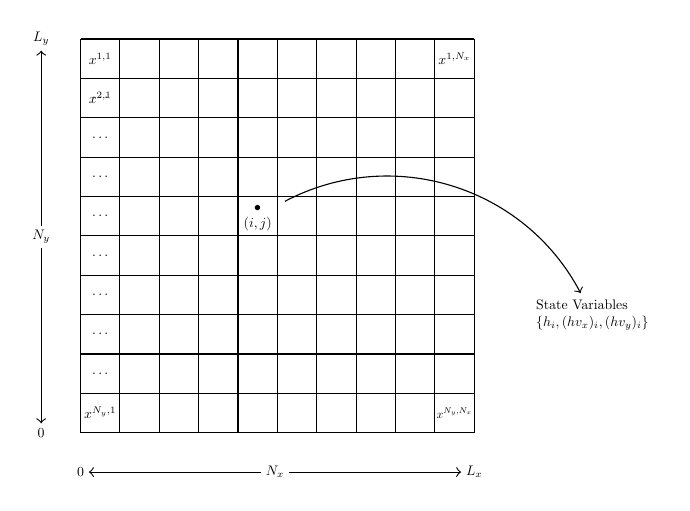
\begin{tikzpicture}[scale=0.5, every node/.style={transform shape}]
\foreach \x in {0,1,2,...,10}
\draw (\x,0) -- (\x,10);
\foreach \x in {0,1,2,...,10}
\draw (0,\x) -- (10,\x);
\node at (0.5,9.5){$x^{1,1}$};
\node at (0.5,8.5){$x^{2,1}$};
\foreach \x in {1,2,...,8}
\node at (0.5,\x+0.5){$\ldots$};
\node at (0.5,0.5){$x^{N_y,1}$};
\node at (9.5,9.5){$x^{1,N_x}$};
\node at (9.5,0.5)[scale=0.86]{$x^{N_y,N_x}$};
\node (A) at (0,-1){0};
\node (B) at (10,-1){$L_x$};
\node (C) at (-1,0){0};
\node (D) at (-1,10){$L_y$};
\draw[<->](A) -- (B)node[midway,fill=white]{$N_x$};
\draw[<->](C) -- (D)node[midway,fill=white]{$N_y$};
\node (E) at (4.5,5.5){\begin{tabular}{c}
$\bullet$ \\ 
$(i,j)$
\end{tabular}};
\node (F) at (13,3){\begin{tabular}{l} 
State Variables \\
$ \lbrace h_i,(hv_x)_i,(hv_y)_i \rbrace $
\end{tabular}};
\draw[->](E) to [bend left=45](F);
\end{tikzpicture}
\caption{$\textbf{X}$: Grid representation of DEM}
\label{grid_dem}
\end{center}
\end{figure}

\subsection{Uncertainty Modeling of the DEM}
\label{dem:uncertainty_model}
Uncertainty model of the DEM has to be accurate to enable an accurate estimation in the variation of the PHM. Modeling the spatial correlation in DEM requires modeling the difference or error maps~\cite{ehlschlaeger1994uncertainty, stefanescu2012digital}. Due to the continuous nature of the actual terrain profile, it is imperative to model the terrain profile as a random field.

In the problem considered in this work, the terrain profile $D$ is modeled as a \textit{second order} Gaussian random field defined on $(\Omega_D, \mathcal{A}, P)$ such that:

\begin{equation}
|| D ||^2_{L_2 (\Omega_D, P)} = \int_{\Omega_D} D^2 dP(\tau) < \infty
\end{equation}

$D$ is characterized by a bounded symmetric and positive definite covariance function $C(\textbf{s})$ with $\textbf{s} \in \Omega_D$ given as,

\begin{equation}
C(\textbf{s}_1, \textbf{s}_2) = \exp{\left( \frac{\textbf{s}_1 - \textbf{s}_2}{a} \right)} \hspace{5mm} \textbf{s}_1, \textbf{s}_2 \in \Omega_D
\end{equation}

\subsection{Adjacency  Matrix and Clustering of Spatial Domain}
\label{dem_adjacency}
The solution of Equation~\ref{main_eq} (Section~\ref{governing}) is achieved by Finite Volume Method. The solution procedure involves discretizing the spatial domain into uniform or non-uniform grid and the equation is then solved on the cell-averages of each grid. For the purpose of computing the adjacency matrix, a uniform grid $\lbrace N_x, N_y \rbrace$ is used. This reduces the PDE in Equation~\ref{main_eq} to a system of Matrix Differential Equation (MDE) involving $3N_x N_y$ variables given as:

\begin{equation}
\label{mde}
\dot{\textbf{Y}} = f(\textbf{Y, D})
\end{equation}

\noindent where, $\textbf{Y} = [\textbf{H}, \textbf{HV}_x, \textbf{HV}_y]^T \in \mathbb{R}^{3N_x \times N_y}$ is the matrix involving the discretized state space. $\textbf{D} \in \mathbb{R}^{N_x \times N_y}$ is the discretized DEM profile, where each cell corresponds to the height of the terrain profile in the discretized domain. The function $f:\mathbb{R}^{3N_x \times N_y} \times \mathbb{R}^{N_x \times N_y} \rightarrow \mathbb{R}^{3N_x \times N_y}$ is implicitly dependent on $\textbf{D}$. The MDE representation in Equation~\ref{mde} is used to compute the adjacency matrix using the concept of statistical linearization~\cite{Mukherjee_2017,roberts2003random,banaszuk2011scalable}. To implement the linearization technique, the 2-D domain $\textbf{X}$ is vectorized to a 1-D domain of length $N = N_x N_y$ as depicted in  Figure~\ref{grid_vec}. Equation~\ref{mde} is vectorized using the \textit{vec} operator as:

\begin{equation}
\label{ode}
vec(\dot{\textbf{Y}}) = vec\left(f(\textbf{Y}, \textbf{D}) \right) = g(vec(\textbf{X}), vec(\textbf{D}))
\end{equation}

\noindent Equation~\ref{ode} is a system of ODE in $\mathbb{R}^{3N}$. To compute the adjacency, following relations are introduced. 
\begin{equation}
\begin{array}{c}
\textbf{Y}_1 = \textbf{H} \hspace{5mm} \textbf{X}_2 = \textbf{HV}_x \hspace{5mm} \textbf{Y}_3 = \textbf{HV}_y \\
\textbf{Y} = [\textbf{Y}_1, \textbf{Y}_2, \textbf{Y}_3] \hspace{5mm} g(\textbf{Y},\textbf{D}) = [g_1(\textbf{Y}_1,\textbf{D}), g(\textbf{Y}_2,\textbf{D}), g(\textbf{X}_3,\textbf{D})]^T
\end{array}
\end{equation}

\begin{figure}
\begin{center}
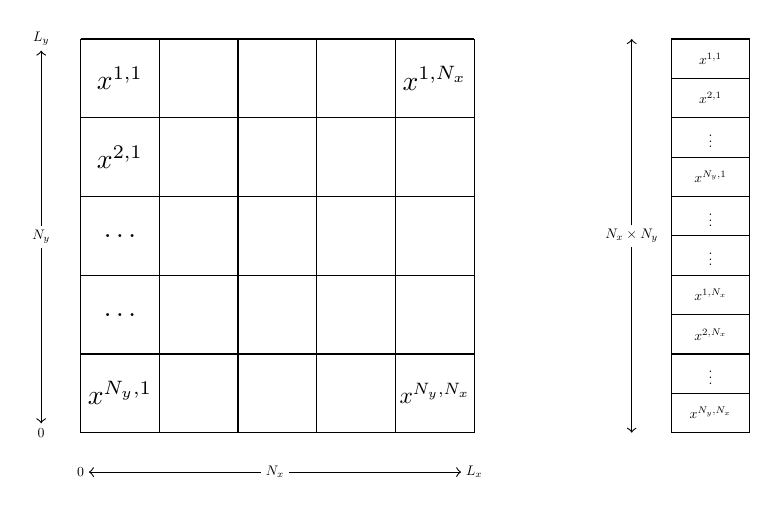
\begin{tikzpicture}[scale=0.5, every node/.style={transform shape}]
\foreach \x in {0,2,4,...,10}
\draw (\x,0) -- (\x,10);
\foreach \x in {0,2,4,...,10}
\draw (0,\x) -- (10,\x);
\node at (1,9)[scale=2]{$x^{1,1}$};
\node at (1,7)[scale=2]{$x^{2,1}$};
\node at (1,5)[scale=2]{$\ldots$};
\node at (1,3)[scale=2]{$\ldots$};
\node at (1,1)[scale=2]{$x^{N_y,1}$};
\node at (9,9)[scale=2]{$x^{1,N_x}$};
\node at (9,1)[scale=1.7]{$x^{N_y,N_x}$};
\node (A) at (0,-1){0};
\node (B) at (10,-1){$L_x$};
\node (C) at (-1,0){0};
\node (D) at (-1,10){$L_y$};
\draw[<->](A) -- (B)node[midway,fill=white]{$N_x$};
\draw[<->](C) -- (D)node[midway,fill=white]{$N_y$};
\foreach \x in {0,1,2,...,10}
\draw (15,\x) -- (17,\x);
\foreach \x in {15,17}
\draw (\x,0) -- (\x,10);
\node at (16,9.5){$x^{1,1}$};
\node at (16,8.5){$x^{2,1}$};
\node at (16,7.5){$\vdots$};
\node at (16,6.5){$x^{N_y,1}$};
\node at (16,5.5){$\vdots$};
\node at (16,4.5){$\vdots$};
\node at (16,3.5){$x^{1,N_x}$};
\node at (16,2.5){$x^{2,N_x}$};
\node at (16,1.5){$\vdots$};
\node at (16,0.5){$x^{N_y,N_x}$};
\draw[<->](14,0) -- (14,10)node[midway,fill=white]{$N_x \times N_y$};
\end{tikzpicture}
\caption{Grid to Vectorization of $\textbf{X}$}
\label{grid_vec}
\end{center}
\end{figure}

\noindent The definition of $g_1(\cdot), g_2(\cdot)$ and $g_3(\cdot)$ follows from the definition of $\textbf{F}, \textbf{G}$ and $\textbf{S}$ in Equation~\ref{defs}. To compute the adjacency, the approximate linear system matrix incorporating the information from $\textbf{X}_1, \textbf{X}_2$ and $\textbf{X}_3$ is given as,

\begin{equation}
\textbf{A}_{sl} = \sum_i^3 \int_{\Omega_{\textbf{D}}} \bigg| \frac{\partial g_i(vec(\textbf{Y}_i),vec(\textbf{D}_w))}{\partial vec(\textbf{Y}_i)} \bigg|_{vec(\textbf{X}_i) = vec(\textbf{X}_i)_0} dP_{\textbf{D}}(\textbf{D}_w) 
\end{equation}

Normalizing and symmetrizing the linear system $A$ results in the adjacency matrix $W$:

\begin{equation}
\label{adj_mat}
\textbf{W} = 0.5\textbf{R}^{-1}(\textbf{A}_{sl} + \textbf{R}\textbf{A}_{sl}^T \textbf{R}^{-1})
\end{equation}

\noindent where, $\textbf{R}$ is the degree matrix for $\textbf{A}_{sl}$. The clustering is performed by solving the following optimization problem~\cite{xie2013overlapping}

\begin{equation}
\label{louvain}
\begin{array}{rl}
\displaystyle \min_{\textbf{Z}} & Q_{ov}  = \frac{1}{2m}\sum_i \sum_{i,j \in c} \left[ A_{i,j} - \frac{k_i k_j}{2m} \right] z_{ic} z_{jc} \\
\displaystyle \text{subject to } & 0 \leq a_{ic} \leq 1 \hspace{5mm} \forall i \in V, \forall c \in C \\
& \displaystyle \sum_c^{|C|} a_{ic} = 1
\end{array}
\end{equation}

\noindent where $C = \lbrace c_1, c_2, \ldots, c_{|C|} \rbrace$ is the set of clusters and $\textbf{Z} = [a_{ij}]_{N \times |C|}$ determines the association of each state $i$ in cluster $j$. $Q_{ov}$ is an overlapping extension of the louvain-modularity function~\cite{blondel2008fast}. Each row of $\textbf{Z}$ corresponds to a particular region in the spatial domain of $\textbf{D}$. Once the $\textbf{Z}$ matrix is estimated, it is used with a given sampling scheme to generate the random samples for the DEM. 


\subsection{Random Sampling and Propagation}

The random sampling follows from the definition of Strongly Coupled Subsystems (SCSs) of a coupled dynamical system. In a system defined by an ode $\dot{\textbf{y}} = g(\textbf{y})$, $\textbf{y} \in \mathbb{R}^n$, $g:\mathbb{R}^n \rightarrow \mathbb{R}^n$, SCSs are defined as element of an overlapping partition of $\textbf{y}$ characterized by an association matrix $\textbf{Z}_{\textbf{x}} = \begin{bmatrix}
\textbf{z}_1 & \ldots & \textbf{z}_m
\end{bmatrix}$ as,
\begin{equation}
\label{hadprod}
\textbf{y} = \bigcup_j^m \textbf{x}_j|j \hspace{5mm} \textbf{y} = \sum_j^m \textbf{z}_j \odot \textbf{y}_j \hspace{5mm} \textbf{y}_j = \begin{bmatrix} \textbf{y}_j|j^T & \textbf{y}_j|j'^T \end{bmatrix}^T \in \mathbb{R}^n
\end{equation}

\noindent such that the SCS $\textbf{y}_j|j \in \mathbb{R}^{n_j}$ can be propagated in parallel and the manifold is defined by the following set of equations

\begin{equation}
\dot{\textbf{y}}_j|j = g_j (\textbf{y}_j|j) \hspace{5mm} g_j:\mathbb{R}^{n_j} \rightarrow \mathbb{R}^{n_j} \hspace{5mm} j = 1 \text{ to } m \hspace{5mm} \sum_j n_j \geq n
\end{equation}

\noindent At any time instance $t \in [0,\infty)$, the mean and covariance of $\textbf{y}$ is preserved under the Hadamard product relation (Following Equation~\ref{hadprod}) as:

\begin{equation}
\label{had_prod}
\begin{array}{l}
E[\textbf{y}] = \sum_j^m \textbf{z}_j \odot E[\textbf{y}_j|j] \\ 
\textbf{cov}(\textbf{y}) = \sum_j^m (\textbf{z}_j\textbf{z}_j^T) \odot \textbf{cov}(\textbf{y}_j|j)
\end{array}
\end{equation}

$\textbf{Z}_{\textbf{x}}$ is estimated from $g$ and the initial distribution of $\textbf{x}$~\cite{Mukherjee_2017overlap}. An SCS $\textbf{x}_j|j$ is identified from $\textbf{Z}_{\textbf{x}}$ using a threshold value $\epsilon$ as:

\begin{equation}
\label{scs_def}
\textbf{y}_j|j = \lbrace x_i| z_{ij} > \epsilon \rbrace
\end{equation}
In this work, we extend this idea of SCS to sample the DEM based on the cluster structure $\textbf{Z}$ identified in Section~\ref{dem_adjacency}. The nodes in weighted graph defined in Equation~\ref{adj_mat} refers to the cells in the spatially discretized domain of $\textbf{D}$. Thus, an SCS identified (Equation~\ref{scs_def}) will be a collection of cells in the discretized domain corresponding to a geographic region in the $\Omega_{\textbf{D}}$. The domain of DEM $\Omega_D$ and hence $vec(\textbf{D})$ is thus partitioned into $m$ number of SCSs $\Omega_{\textbf{D}_i}$ and $vec(\textbf{D}_i)$ of length $N_j$ such that:

\begin{equation}
\Omega_{\textbf{D}} = \bigcup_j^m \Omega_{\textbf{D}_j} \hspace{5mm} \sum_j N_j \geq N
\end{equation}

This partition can be used to generate realizations of $\textbf{D}$. Instead of sampling the whole DEM, one can sample a single zone $\Omega_{\textbf{D}_i}$, keeping the rest of the DEM at its nominal value. 


\subsection{Sampling of a Zone}

The sampling is done on a subdomain $\Omega_{D_j}$ at a time. The covariance function $C(x,y)$ defined in Section~\ref{dem:uncertainty_model} admits a spectral decomposition as~\cite{ghanem2003stochastic}:

\begin{equation}
\label{cov_int}
C(\textbf{s}_1,\textbf{s}_2) = \sum_{l=0}^\infty \lambda_l f_l(\textbf{s}_1) f_l(\textbf{s}_2) \hspace{5mm} \textbf{s}_1,\textbf{s}_2 \in \Omega_{D_j}
\end{equation}

\noindent where, $\lambda_l$ and $f_l(\textbf{s})$ are solutions to the following integral equation

\begin{equation}
\int_{\Omega_{D_j}} C(\textbf{s}_1,\textbf{s}_2) f_l(\textbf{s}_1)d\textbf{s}_1 = \lambda_l f_l(\textbf{s}_2)
\end{equation}

The variable $D$ for the subdomain $\Omega_{D_j}$ can be written as,

\begin{equation}
\label{kl_full}
D(\textbf{s}) = \mu_D(\textbf{s}) + \sum_{l=0}^\infty \xi_l f_l(\textbf{s}) \hspace{5mm} \xi_l = \int_{\Omega_{D_j}} (D(\textbf{s}) - \mu_D(\textbf{s}) )f_l(\textbf{s})d\textbf{s}
\end{equation}

\noindent where, $\xi_l$ are zero mean uncorrelated random variables with variance as $\lambda_l$. In practice, the summation in Equation~\ref{kl_full} is truncated up to a certain order $M$~\cite{ghanem2003stochastic} as

\begin{equation}
\label{kl_trunc}
D(\textbf{s}) = \mu_D(\textbf{s}) + \sum_{l=0}^M \xi_l f_l(\textbf{s})
\end{equation}

 
Analytical solution to the equation~\ref{cov_int} exists only for certain covariance functions. Numerical methods~\cite{atkinson2009numerical,hansen1992numerical} for solving Equation~\ref{cov_int} involves the evaluating the function $C(\textbf{s})$ for the discretized space $\textbf{X}$ defined in Section~\ref{highres}. This leads to solving the following eigenvalue problem: 

\begin{equation}
\textbf{C}_j\textbf{W}_j \textbf{f}_l = \lambda_l \textbf{f}_l
\end{equation}

\noindent where, $\textbf{C}_j$ and $\textbf{W}_j$ are $N_j \times N_j$ matrices given as


\begin{equation}
\label{cov_mat}
\resizebox{0.9\textwidth}{!}{%
$\textbf{C}_j = \begin{bmatrix}
C(x_j^{1},x_j^{1}) & C(x_j^{1},x_j^{2}) & \ldots & C(x_j^{1},x_j^{N_j}) \\
 & C(x_j^{2},x_j^{2}) & \ldots & C(x_j^{2},x_j^{N_j}) \\
& \vdots & \ddots & \vdots \\
&  &  &   C(x_j^{N_j},x_j^{N_j})
\end{bmatrix}
\textbf{W} = \begin{bmatrix}
1/N_j & 0 & \ldots & 0 \\
& 1/N_j & \ldots & 0 \\
 & \vdots & \ddots & \vdots \\
 & 0 & & 1/N_j
\end{bmatrix}$}
\end{equation}

Once the $M$ eigenvalues $\lambda_l$ and eigenvectors $\textbf{f}_l$'s are computed, sampling of $D$ gets reduced to generating realizations for $M$-dimensional $\xi = \lbrace \xi_1,\xi_2,\ldots, \xi_M \rbrace$.

Although, the above method is easy to implement, it is computationally expensive for high resolution DEMs that encompasses the full domain $\Omega_{D}$. The SCS identification-based method enables to sample the sub-regions in parallel with fewer realizations maintaining the same accuracy. This SCS-based sampling procedure can be used to sample a realization for the whole domain $\Omega_j$ by sampling a single zone $\Omega_j$ at a time. Algorithm~\ref{sample_dem} describes the overall procedure of clustering, sampling, propagation, and estimation of moments for a given cluster structure.


\begin{algorithm}[H]
\caption{Clustering of DEM using SCS and Propagation}
\label{sample_dem}
\begin{algorithmic}
\Require $C_\textbf{D}(x,y)$, $\textbf{Z}$, $N_x$, $N_y$, $\Omega_{\textbf{D}_j}$'s $j = 1$ to $m$
\Ensure $E(\textbf{U})$, $\textbf{cov}(\textbf{U})$ at each time
\ForAll{t}
\ForAll{j}
\State Sample $D_j(\textbf{s}), \textbf{s} \in \Omega_j$ using Equation~\ref{kl_trunc}
\State Create $D$ sample by keeping rest of the zones at $\mu(D)$
\State Propagate Equation~\ref{main_eq} for Zone $j$
\State Compute $E(\textbf{U})$ and $\textbf{cov}(\textbf{U})$ for Zone $j$
\EndFor
\State Compute $E(\textbf{U})$ and $\textbf{cov}(\textbf{U})$ at time $t$ using Equation~\ref{had_prod}
\EndFor
\end{algorithmic}
\end{algorithm}

\section{Generation of Realizations via Sampling Scheme}
\label{dem:uncertainty}
At each time instance, one is interested in computing the statistical properties of the pile height $h$ in Equation~\ref{main_eq} by evaluating multidimensional integral (Equation~\ref{monte_int}) of the form

\begin{equation}
\label{dem_monte_int}
E[h^a] = \int_{\Omega_D}  h^a(D) p_{D}(D) dD \approx  \frac{1}{\mathcal{N}}\sum_i^\mathcal{N} h^a(\mathcal{D}_i)
\end{equation}

The above integral is solved using sampling or quadrature based techniques described in Chapter~\ref{chap:uq}. In this reported work, the Latin Hypercube Sampling method~\cite{iman2008latin} has been used for generating the sampling space to compute the integral Equation~\ref{dem_monte_int}.

\section{Volcanic Locations}
\label{volcanic_location}
To implement the methodology explained in Section~\ref{dem_adjacency}, two volcanic locations are chosen, whereby the simulation of debris or avalanche flow resulting from a volcanic eruption on a realistic topography is demonstrated. For each location, the cluster structure as per Section~\ref{dem_adjacency} is computed and the DEM realizations are generated by Algorithm~\ref{sample_dem}. To understand the dependency of the cluster structure on the resolution $\lbrace N_x, N_y \rbrace$, a comparison of the cluster structure with the resolution of discretization has been performed.
After fixing a cluster structure for a given resolution, it is used to sample realizations.
For each realization in a cluster, the flow equation in~\ref{main_eq} is propagated. The average pile height is computed at each time to construct the PHM.

\subsection{Colima}

The Volcan de Colima~\cite{luhr1981colima} erupted in 1991, creating an impact up to a distance of 4 km. This phenomenon has been studied and simulated several times~\cite{rupp2003colima,pitman2003computing,rupp2006colima}. Figure~\ref{fig:colima} shows the extent of the colima region and the elevation profile of the region of interest. The Colima DEM is a $4.5 \text{km} \times 4.5\text{km}$ control region of resolution $5 \text{m}$. In the current setup, a cylindrical pile deposition of approximately $10^6$ $\text{m}^3$ is considered. The angle of frictions are assumed to be $\phi_{bed} = 27^\circ$ and $\phi_{int} = 37^\circ$. 

\begin{figure}[H]
\begin{subfigure}{0.4\textwidth}
\centering
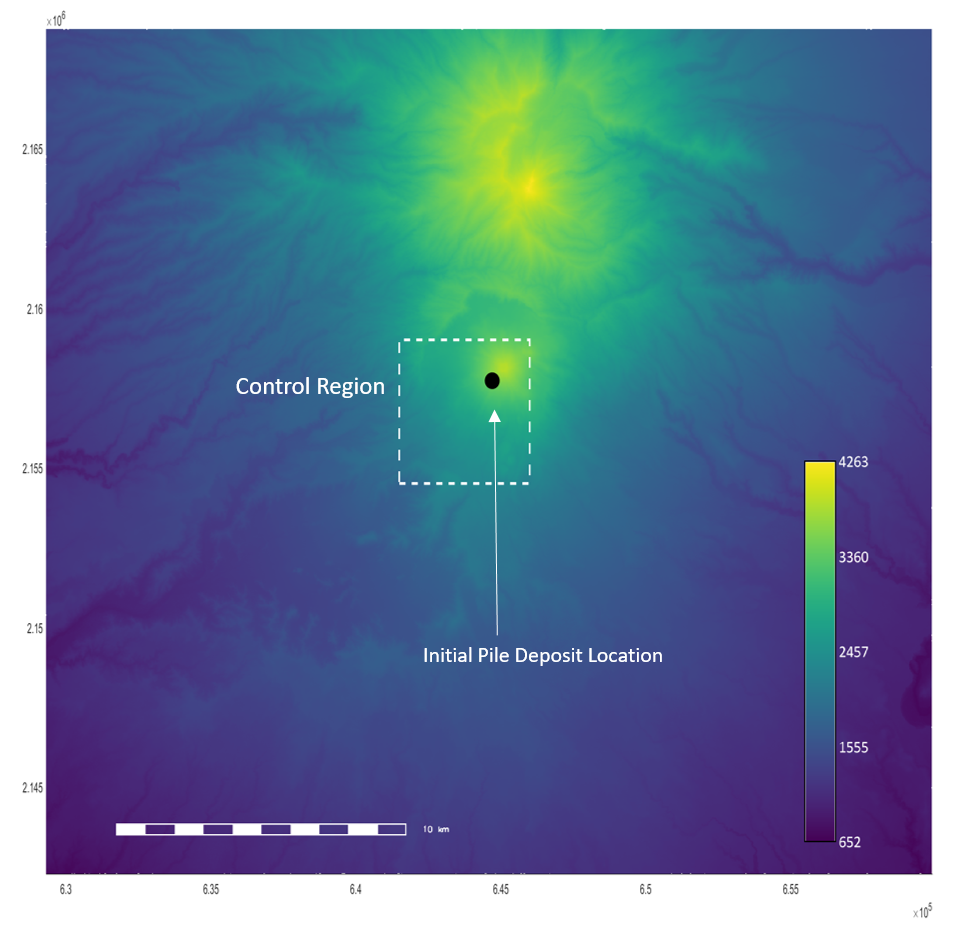
\includegraphics[width=\textwidth]{dem_figs/colima_4}
\caption{}
\label{colima_1}
\end{subfigure}
\centering
\begin{subfigure}{0.55\textwidth}
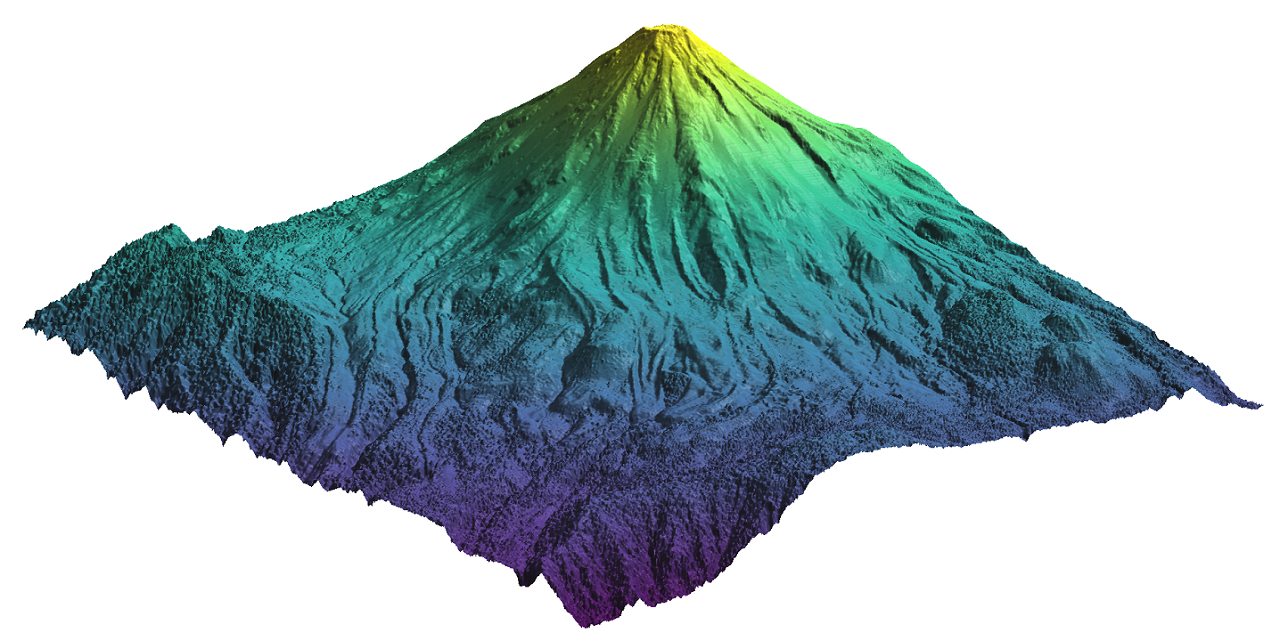
\includegraphics[width=0.9\textwidth]{dem_figs/colima_el}
\caption{}
\label{colima_2}
\end{subfigure}
\caption{Geographic region of Volcan de Colima, showing the (a) control region and initial pile deposit location and (b) the elevation profile of the control region.}
\label{fig:colima}
\end{figure}

The $5m$  DEM is downscaled to different resolutions to compute the adjacency.
Figure~\ref{fig:colima_adjacency} shows the plot of the matrix $W$ for each resolution $\lbrace N_x, N_y\rbrace$. The plots are highly sparse as the resolution increases. Figure~\ref{fig:colima_cluster} shows the clusters detected in the control region. The cluster structure asymptotically converges with the resolution of discretization, and hence the original $5$ m DEM is not required in practice for the cluster generation. Since the cluster boundaries are fairly discernible with in $100$ m and $150$ m DEMs, the higher resolution cluster structure can be well interpolated from these maps. Also, the cluster structure corresponds to different height levels. This shows that the spatial correlation produces better effect on the cluster map. This cluster structure is now used to generate the realizations for each of the zone in parallel. 

\begin{figure}[H]
\begin{subfigure}{0.48\textwidth}
\centering
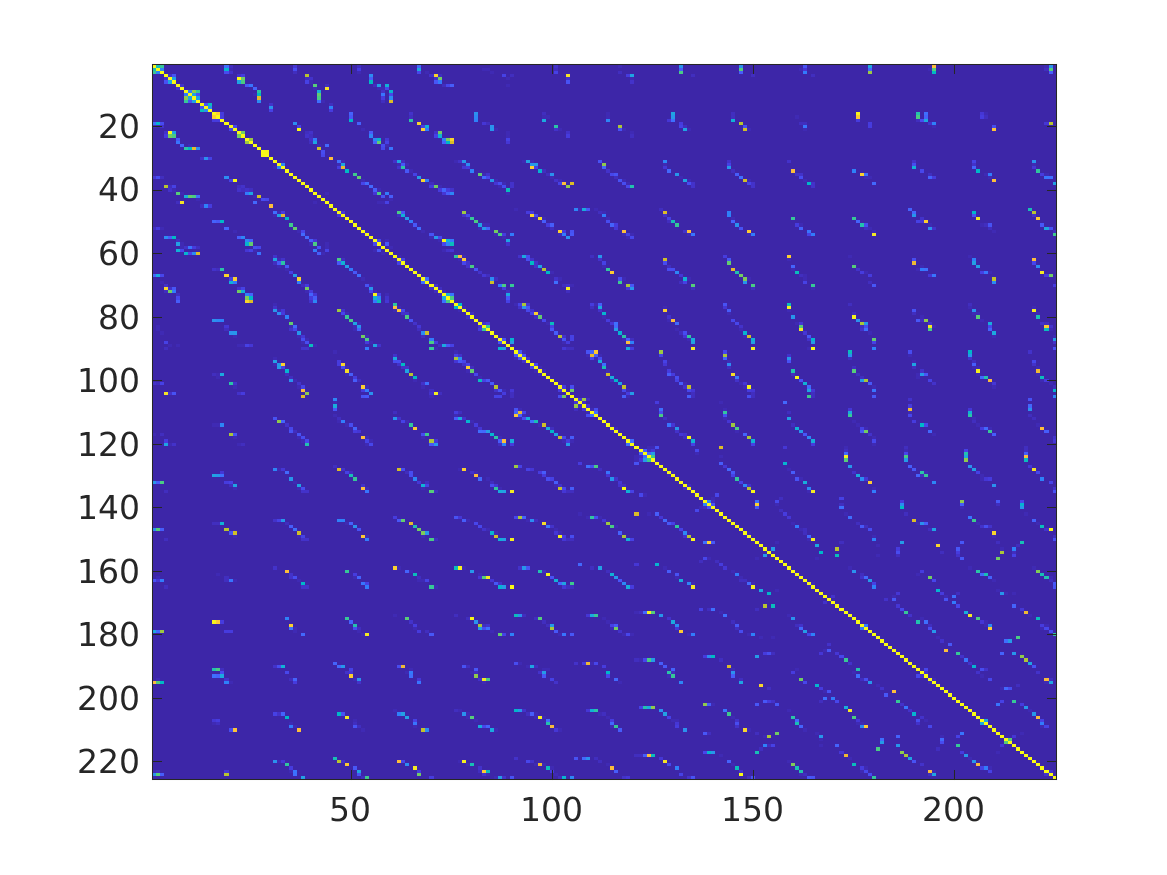
\includegraphics[width=\textwidth]{dem_figs/colima_adjacency_300}
\caption{Adjacency with 300 m resolution}
\label{colima_adjacency_300}
\end{subfigure}
\centering
\begin{subfigure}{0.48\textwidth}
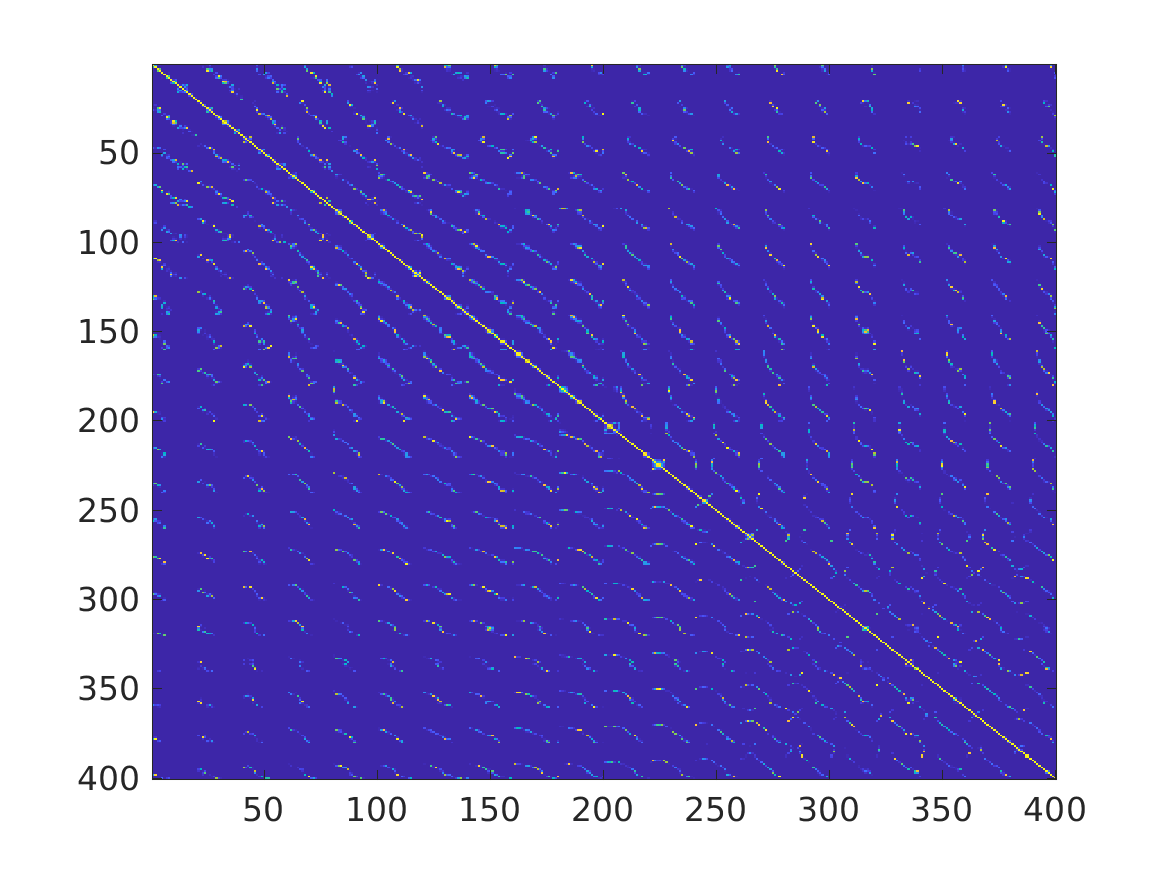
\includegraphics[width=\textwidth]{dem_figs/colima_adjacency_225}
\caption{Adjacency with 225 m resolution}
\label{colima_adjacency_225}
\end{subfigure} \\
\begin{subfigure}{0.48\textwidth}
\centering
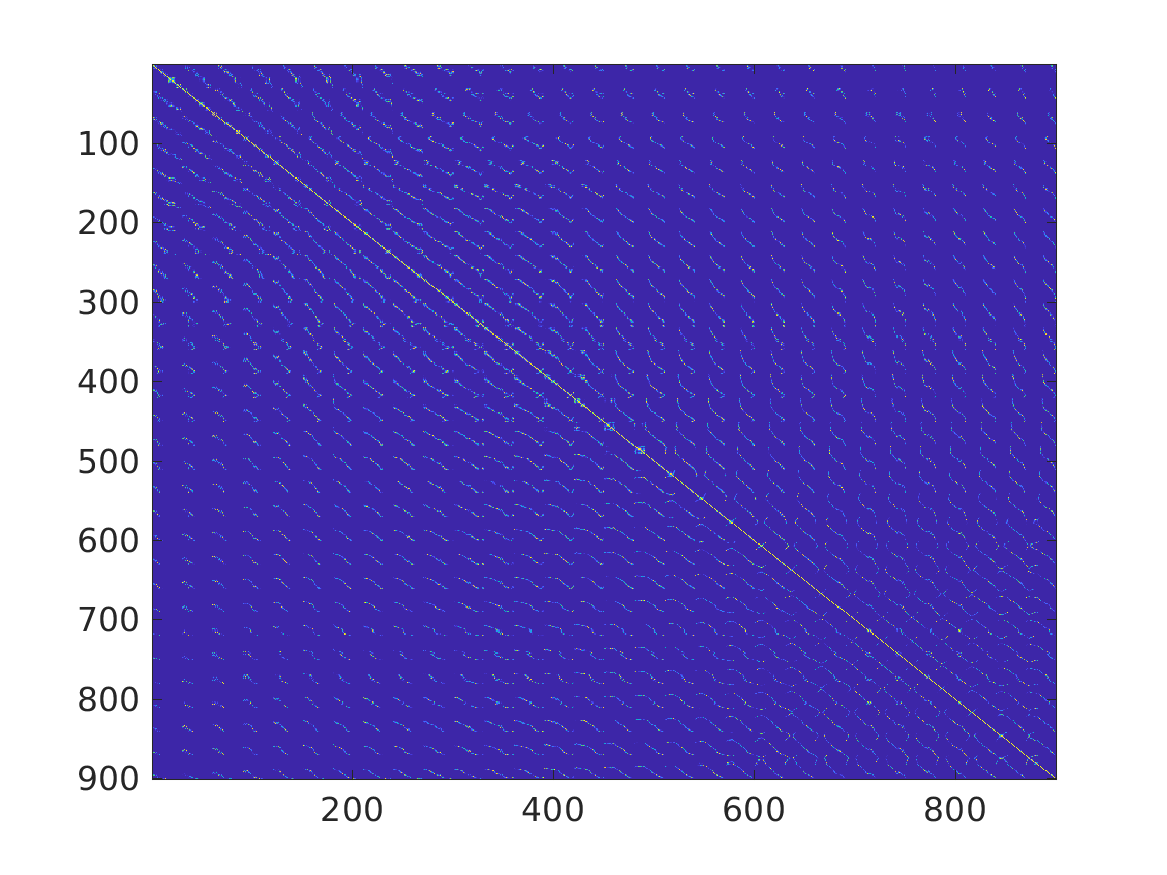
\includegraphics[width=\textwidth]{dem_figs/colima_adjacency_150}
\caption{Adjacency with 150 m resolution}
\label{colima_adjacency_150}
\end{subfigure}
\centering
\begin{subfigure}{0.48\textwidth}
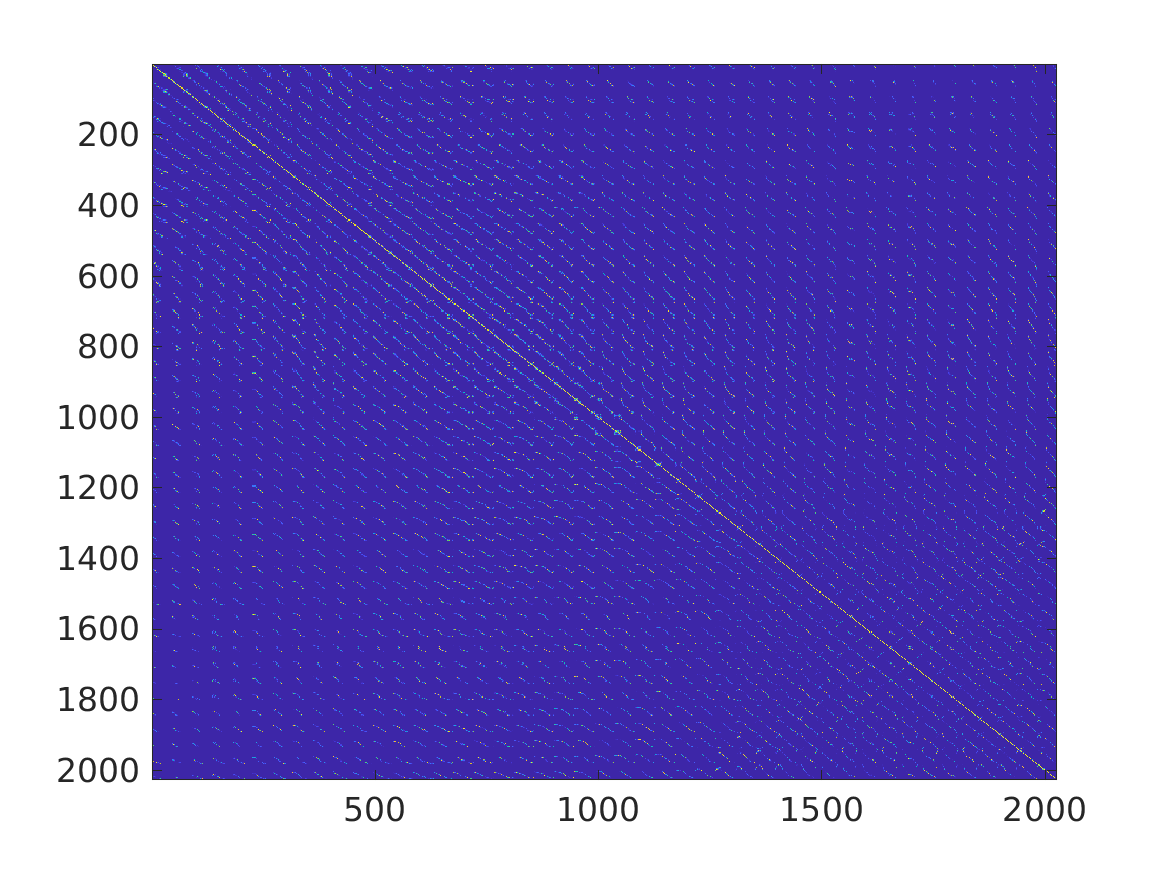
\includegraphics[width=\textwidth]{dem_figs/colima_adjacency_100}
\caption{Adjacency with 100 m resolution}
\label{colima_adjacency_100}
\end{subfigure} 
\caption{Adjacency Matrix for Volcan de Colima using different resolutions of discretization.}
\label{fig:colima_adjacency}
\end{figure}

\begin{figure}[H]
\begin{subfigure}{0.48\textwidth}
\centering
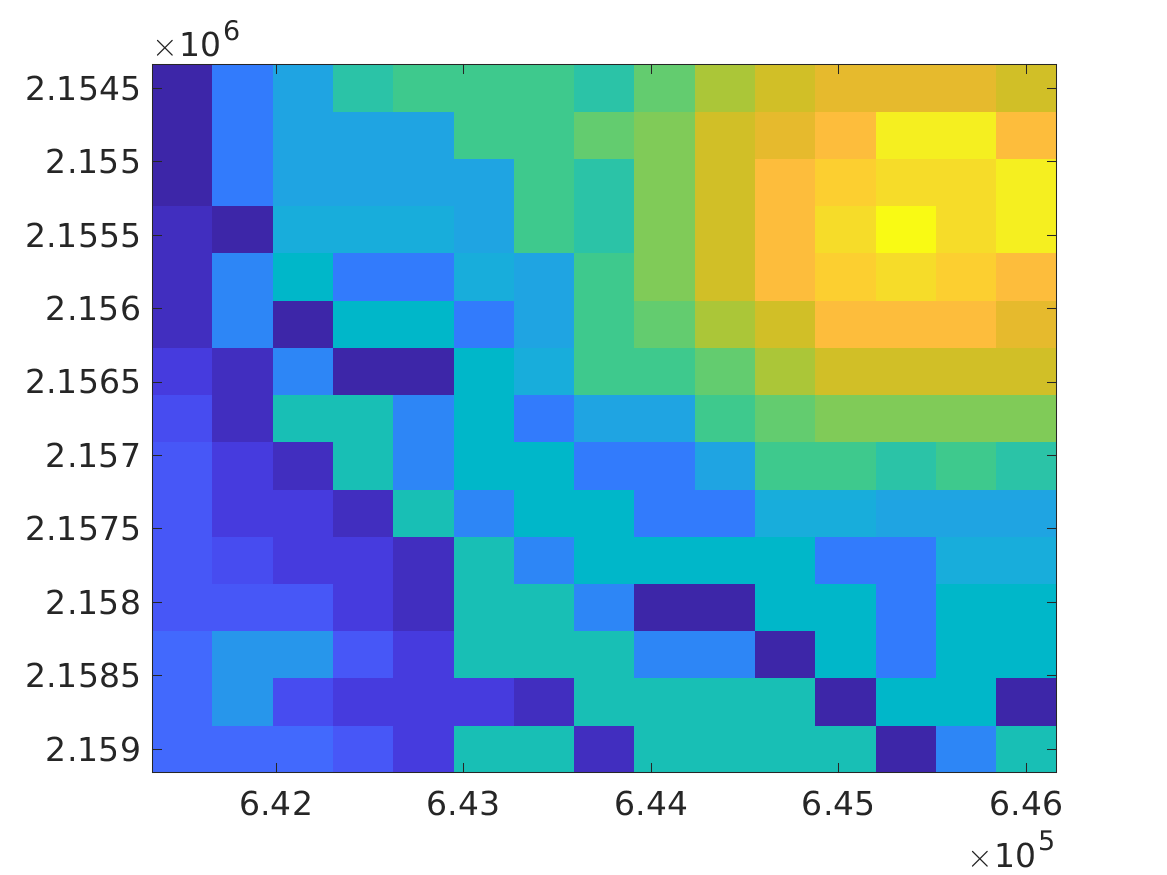
\includegraphics[width=\textwidth]{dem_figs/colima_cluster_300}
\caption{Cluster structure with 300 m resolution}
\label{colima_cluster_300}
\end{subfigure}
\centering
\begin{subfigure}{0.48\textwidth}
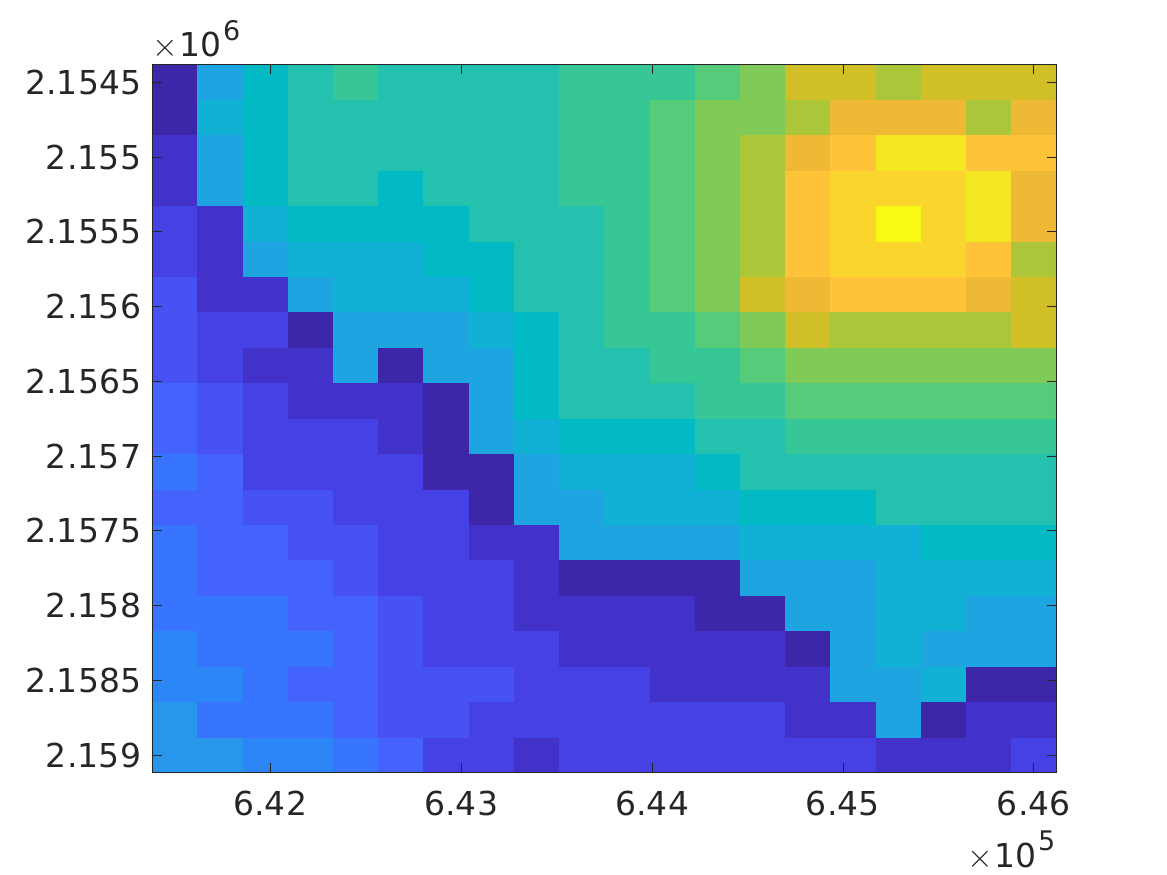
\includegraphics[width=\textwidth]{dem_figs/colima_cluster_225}
\caption{Cluster structure with 225 m resolution}
\label{colima_cluster_225}
\end{subfigure} \\
\begin{subfigure}{0.48\textwidth}
\centering
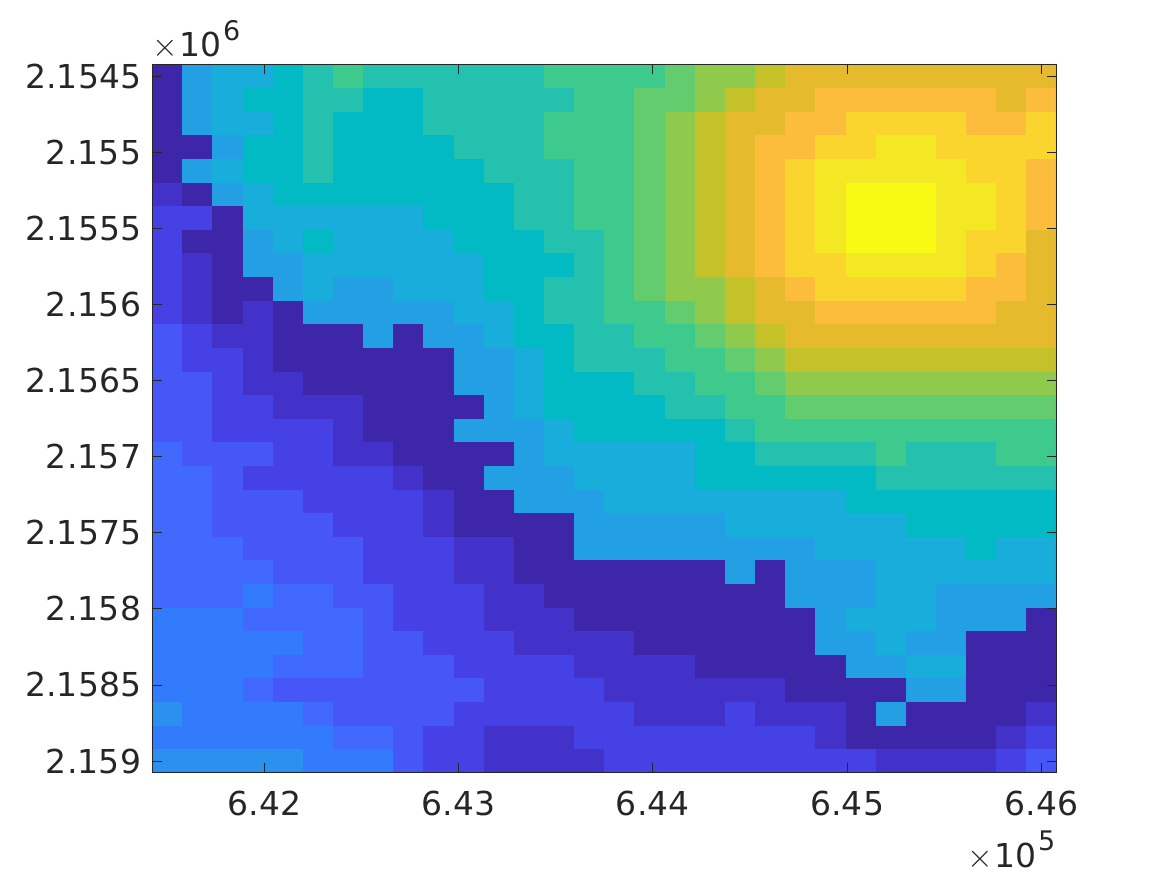
\includegraphics[width=\textwidth]{dem_figs/colima_cluster_150}
\caption{Cluster structure with 150 m resolution}
\label{colima_cluster_150}
\end{subfigure}
\centering
\begin{subfigure}{0.48\textwidth}
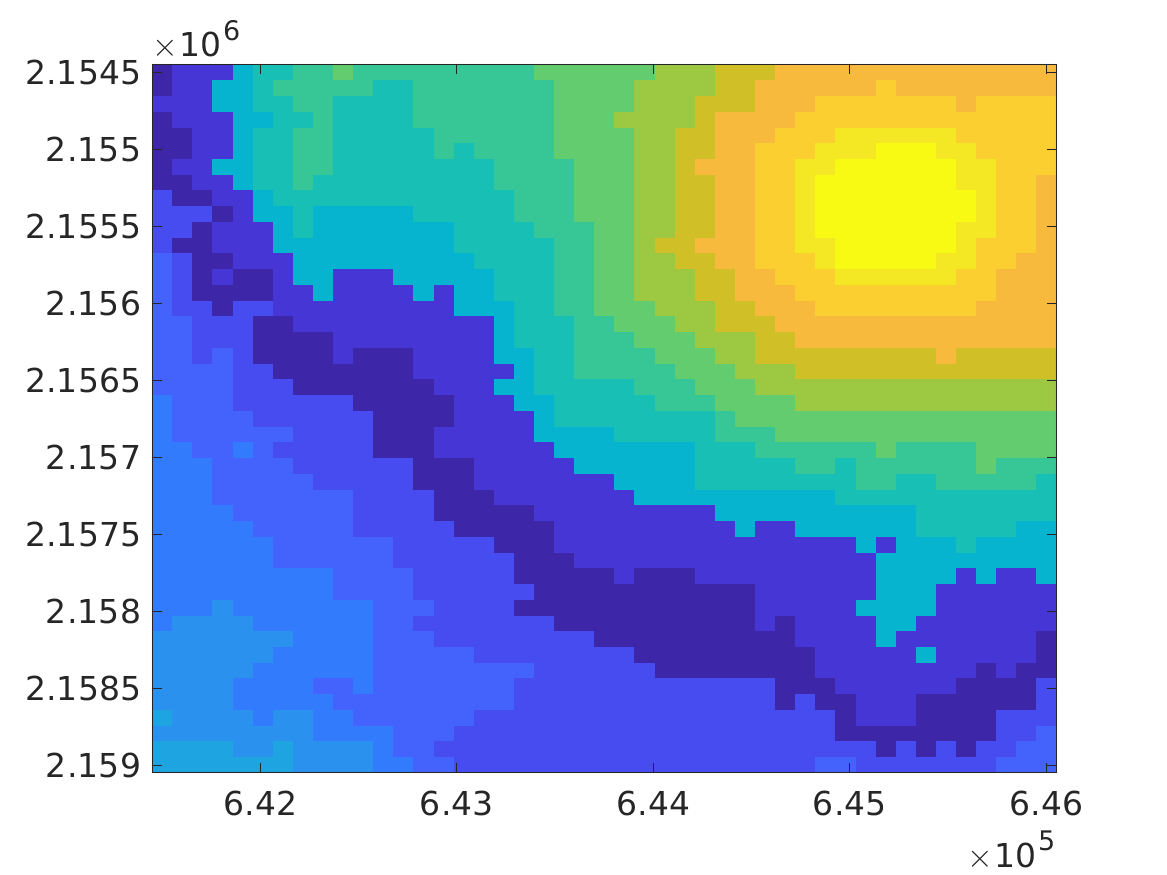
\includegraphics[width=\textwidth]{dem_figs/colima_cluster_100}
\caption{Cluster structure with 100 m resolution}
\label{colima_cluster_100}
\end{subfigure} 
\caption{Cluster structure for Volcan de Colima using different resolutions of discretization.}
\label{fig:colima_cluster}
\end{figure}

Figure~\ref{fig:colima_simulate} shows the mean pile height $E(\textbf{U})$ at different time instance of the simulation. The hazard flow (in blue) is represented on a gray-scale image of the volcanic location to show its spread. The mean height is calculated for each zone in parallel and then the overall height is computed using the Hadamard product formula of Equation~\ref{had_prod}.

\begin{figure}[H]
\centering
\begin{subfigure}{0.46\textwidth}
\centering
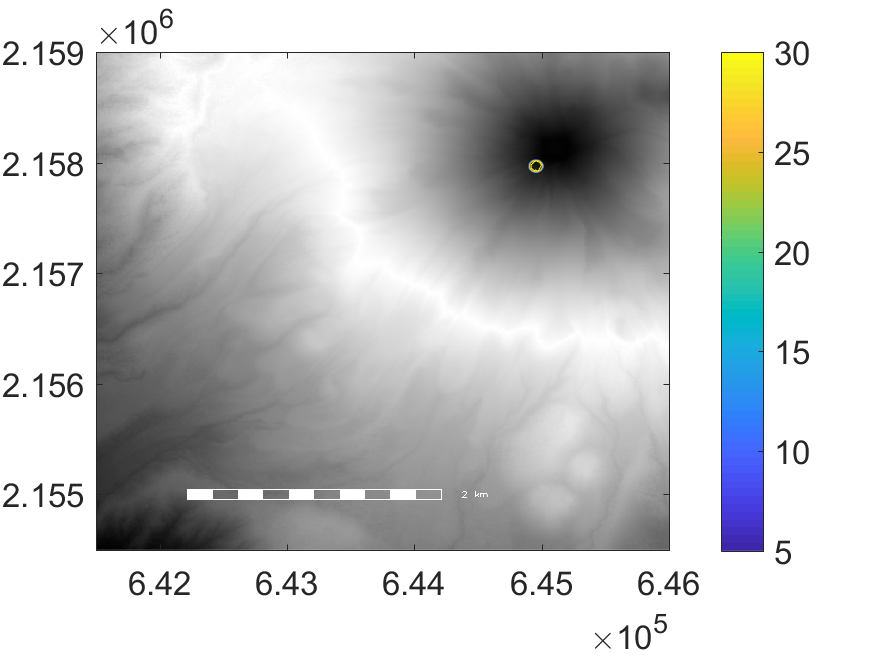
\includegraphics[width=\textwidth]{dem_figs/newres_1}
\caption{at Time = 1s}
\end{subfigure}
\begin{subfigure}{0.46\textwidth}
\centering
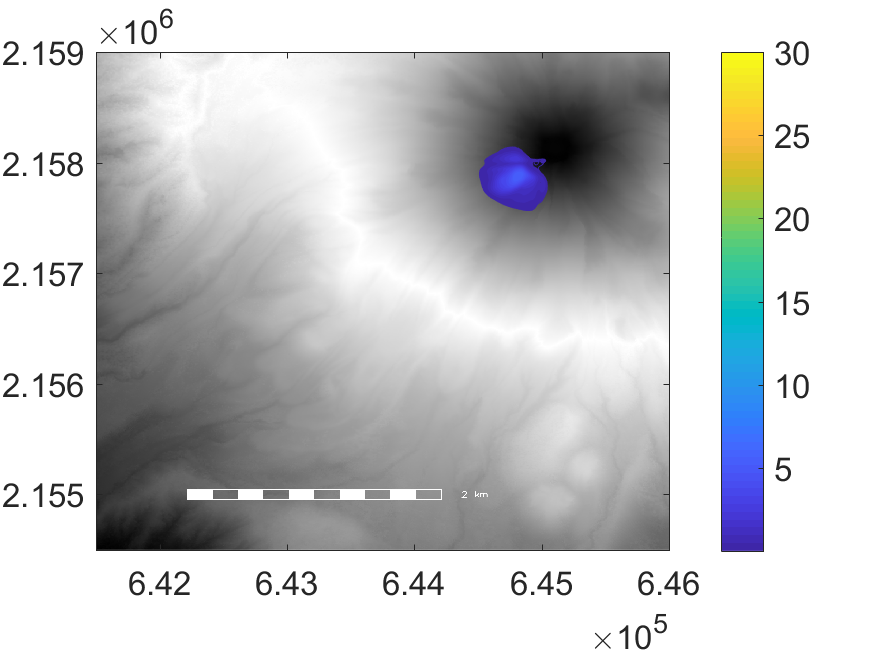
\includegraphics[width=\textwidth]{dem_figs/newres_13}
\caption{at Time = 13s} 
\end{subfigure} \\
\begin{subfigure}{0.46\textwidth}
\centering
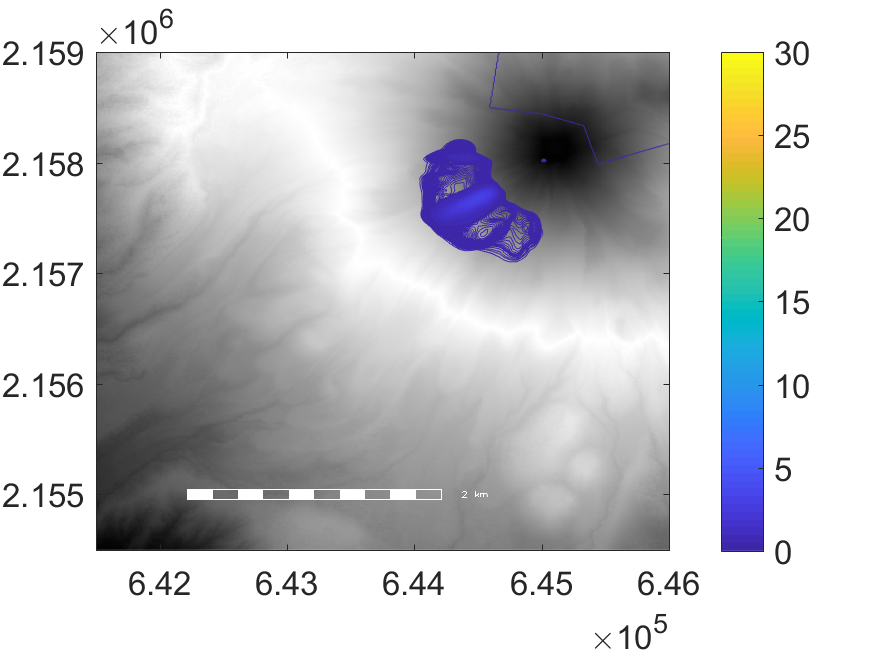
\includegraphics[width=\textwidth]{dem_figs/newres_25}
\caption{at Time = 25s}
\end{subfigure}
\begin{subfigure}{0.46\textwidth}
\centering
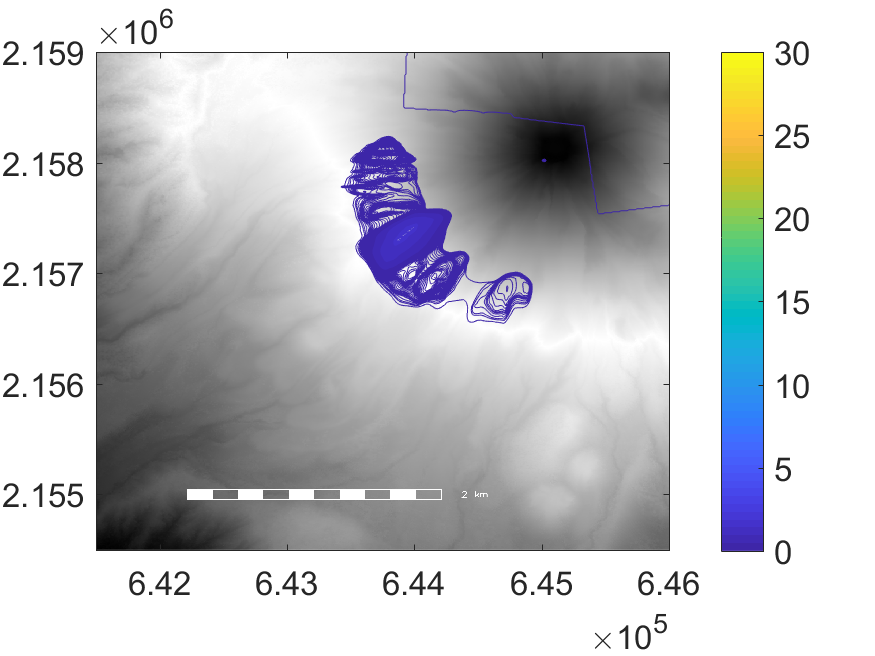
\includegraphics[width=\textwidth]{dem_figs/newres_37}
\caption{at Time = 37s}
\end{subfigure}
\caption{Mean Pile height at different time instance}
\label{fig:colima_simulate}
\end{figure}

To establish the accuracy of the SCS-based UQ, error plots have been plotted. A full model sampling space has been generated using Latin-Hypercube sampling. Spatial error in terms of the average pile height between the full model and the SCS-based model has been computed using the metric given as:

\begin{equation}
\epsilon_{\textbf{U}} = \frac{|E(\textbf{U})_c - E(\textbf{U})_f|}{\max_{\Omega_{D}} (E(\textbf{U})_f)}
\end{equation}

\noindent where, $E(\textbf{U})_c$ is computed from the SCS-based model and $E(\textbf{U})_f$ is computed from the full sampling scheme. Figure~\ref{fig:colima_error} shows the plot of $\epsilon_{\textbf{U}}$ for the volcanic region at different time instance. The color-bar at the side of each plots show the range of the value. The normalized error value ranges from 0.01 to 0.14 establishing the high efficiency of the SCS-based method in maintaining the accuracy of PHM estimation for a parallel sampling scheme. 


\begin{figure}[H]
\centering
\begin{subfigure}{0.46\textwidth}
\centering
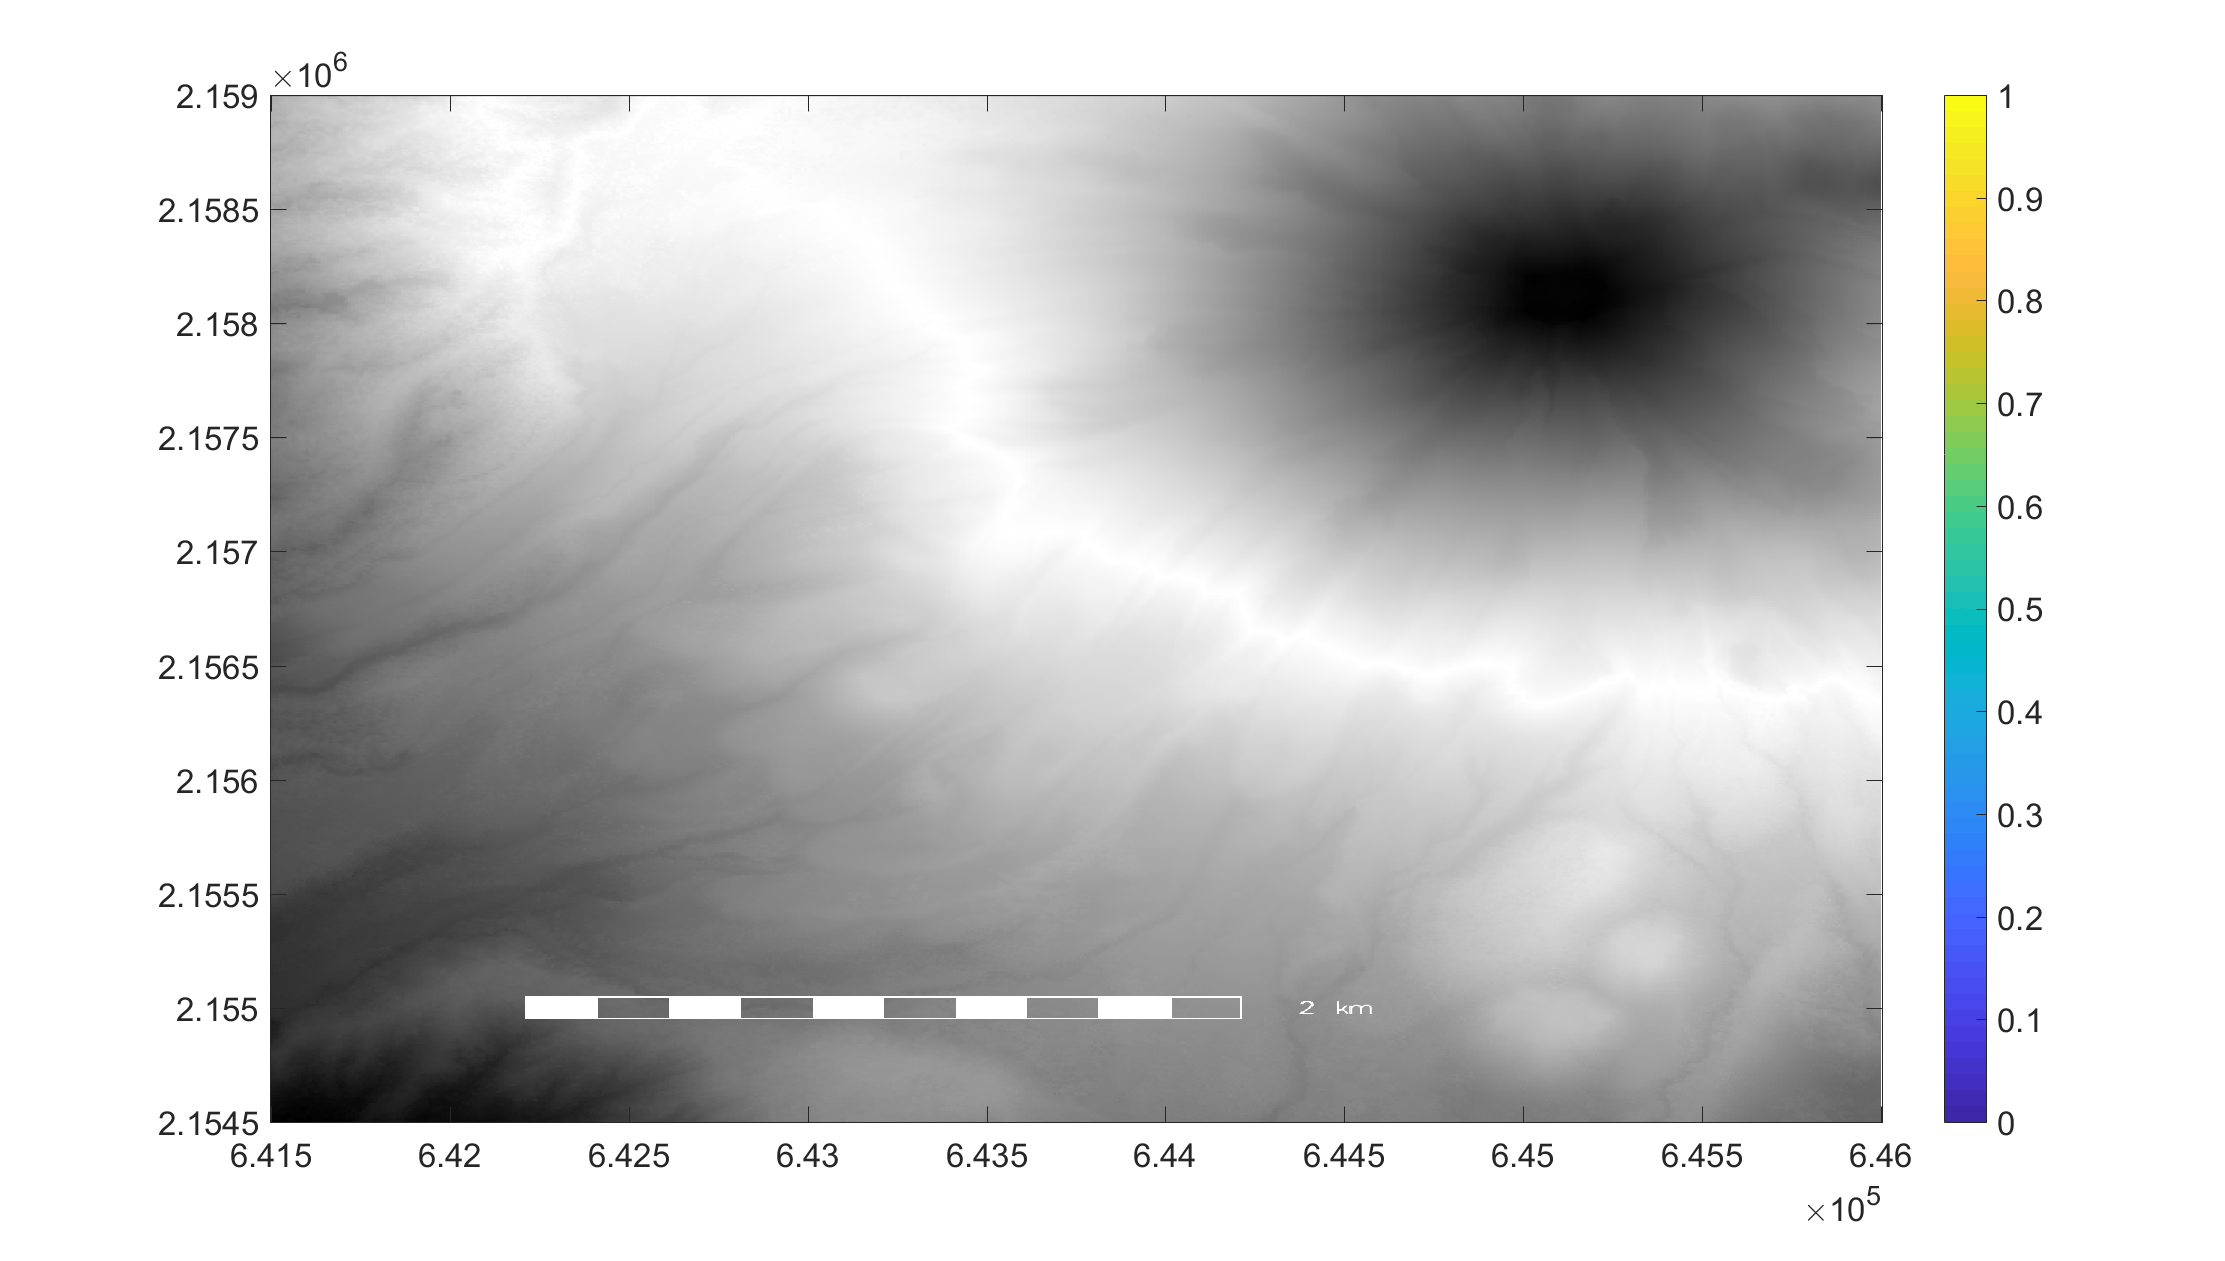
\includegraphics[width=\textwidth]{dem_figs/fig1}
\caption{at Time = 1s}
\end{subfigure}
\begin{subfigure}{0.46\textwidth}
\centering
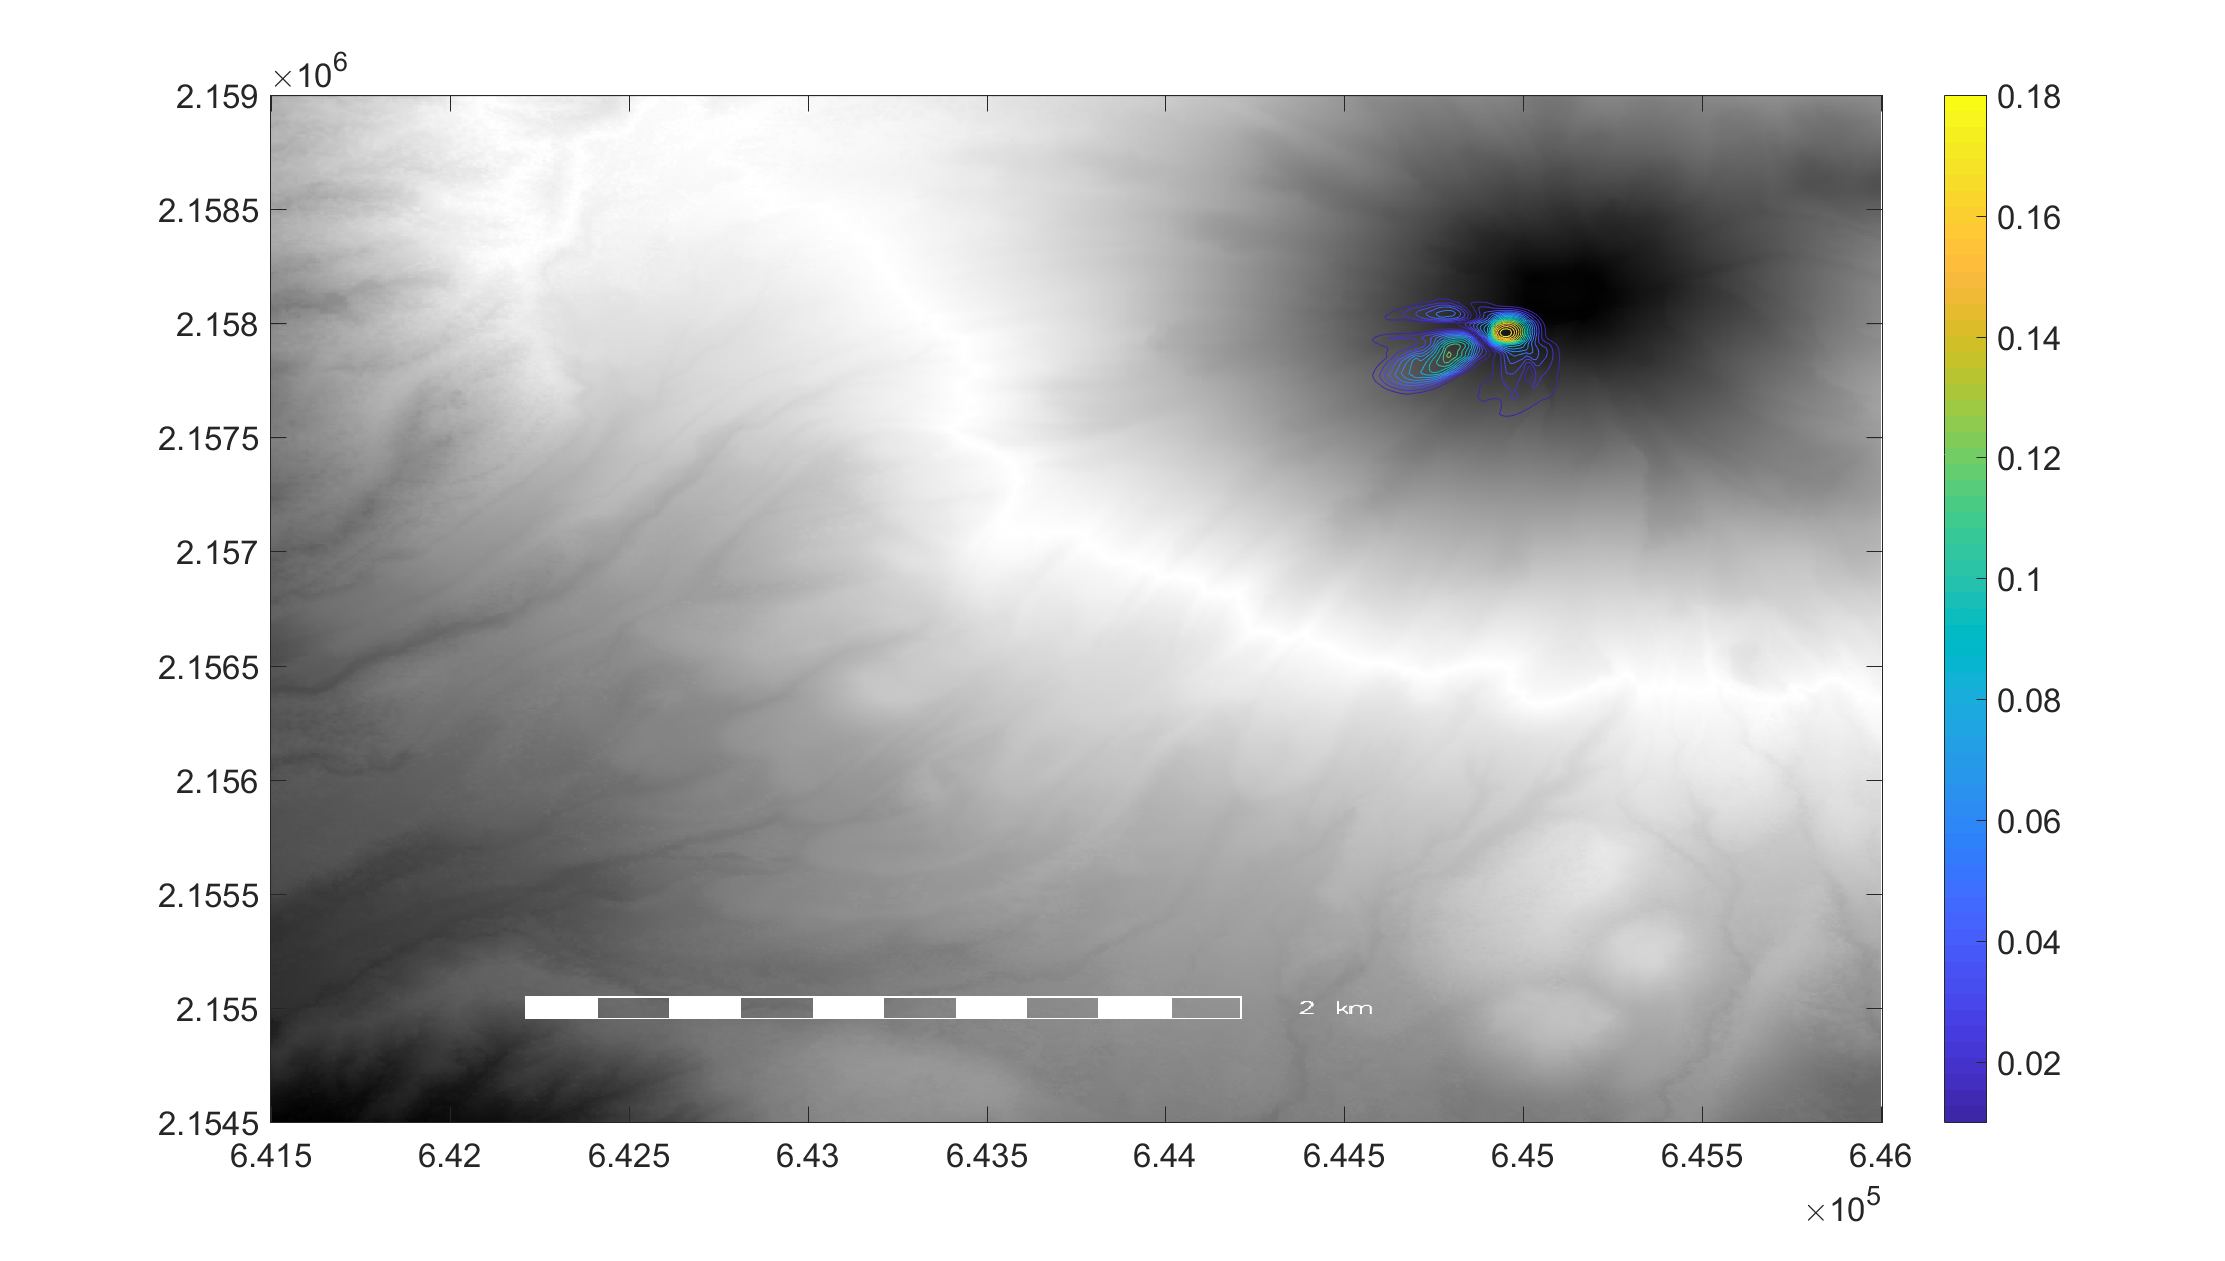
\includegraphics[width=\textwidth]{dem_figs/fig13}
\caption{at Time = 13s} 
\end{subfigure} \\
\begin{subfigure}{0.46\textwidth}
\centering
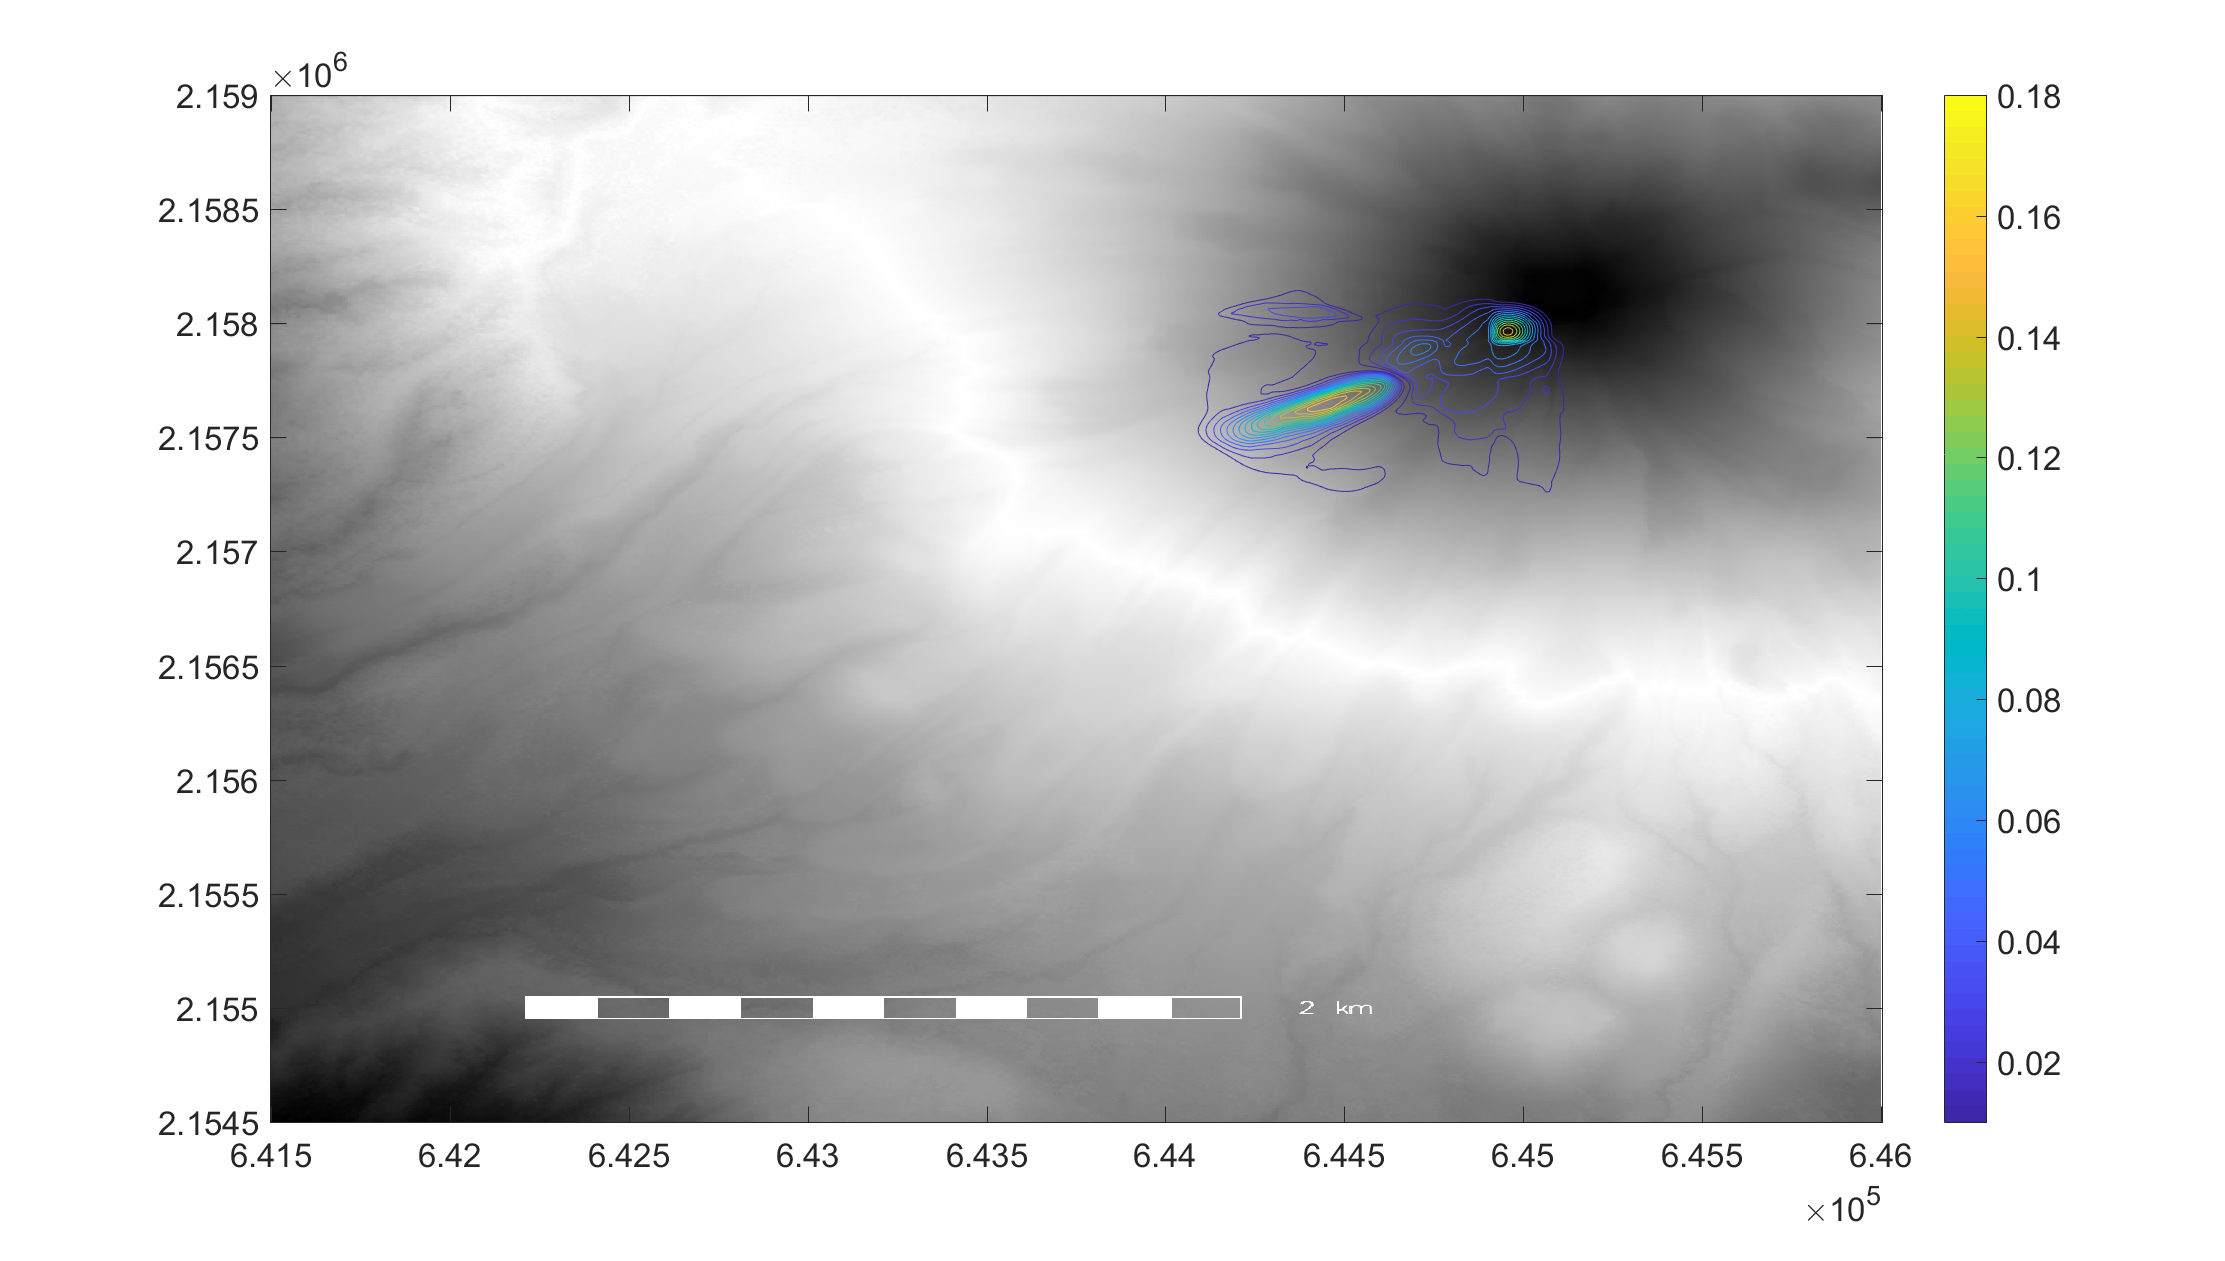
\includegraphics[width=\textwidth]{dem_figs/fig25}
\caption{at Time = 25s}
\end{subfigure}
\begin{subfigure}{0.46\textwidth}
\centering
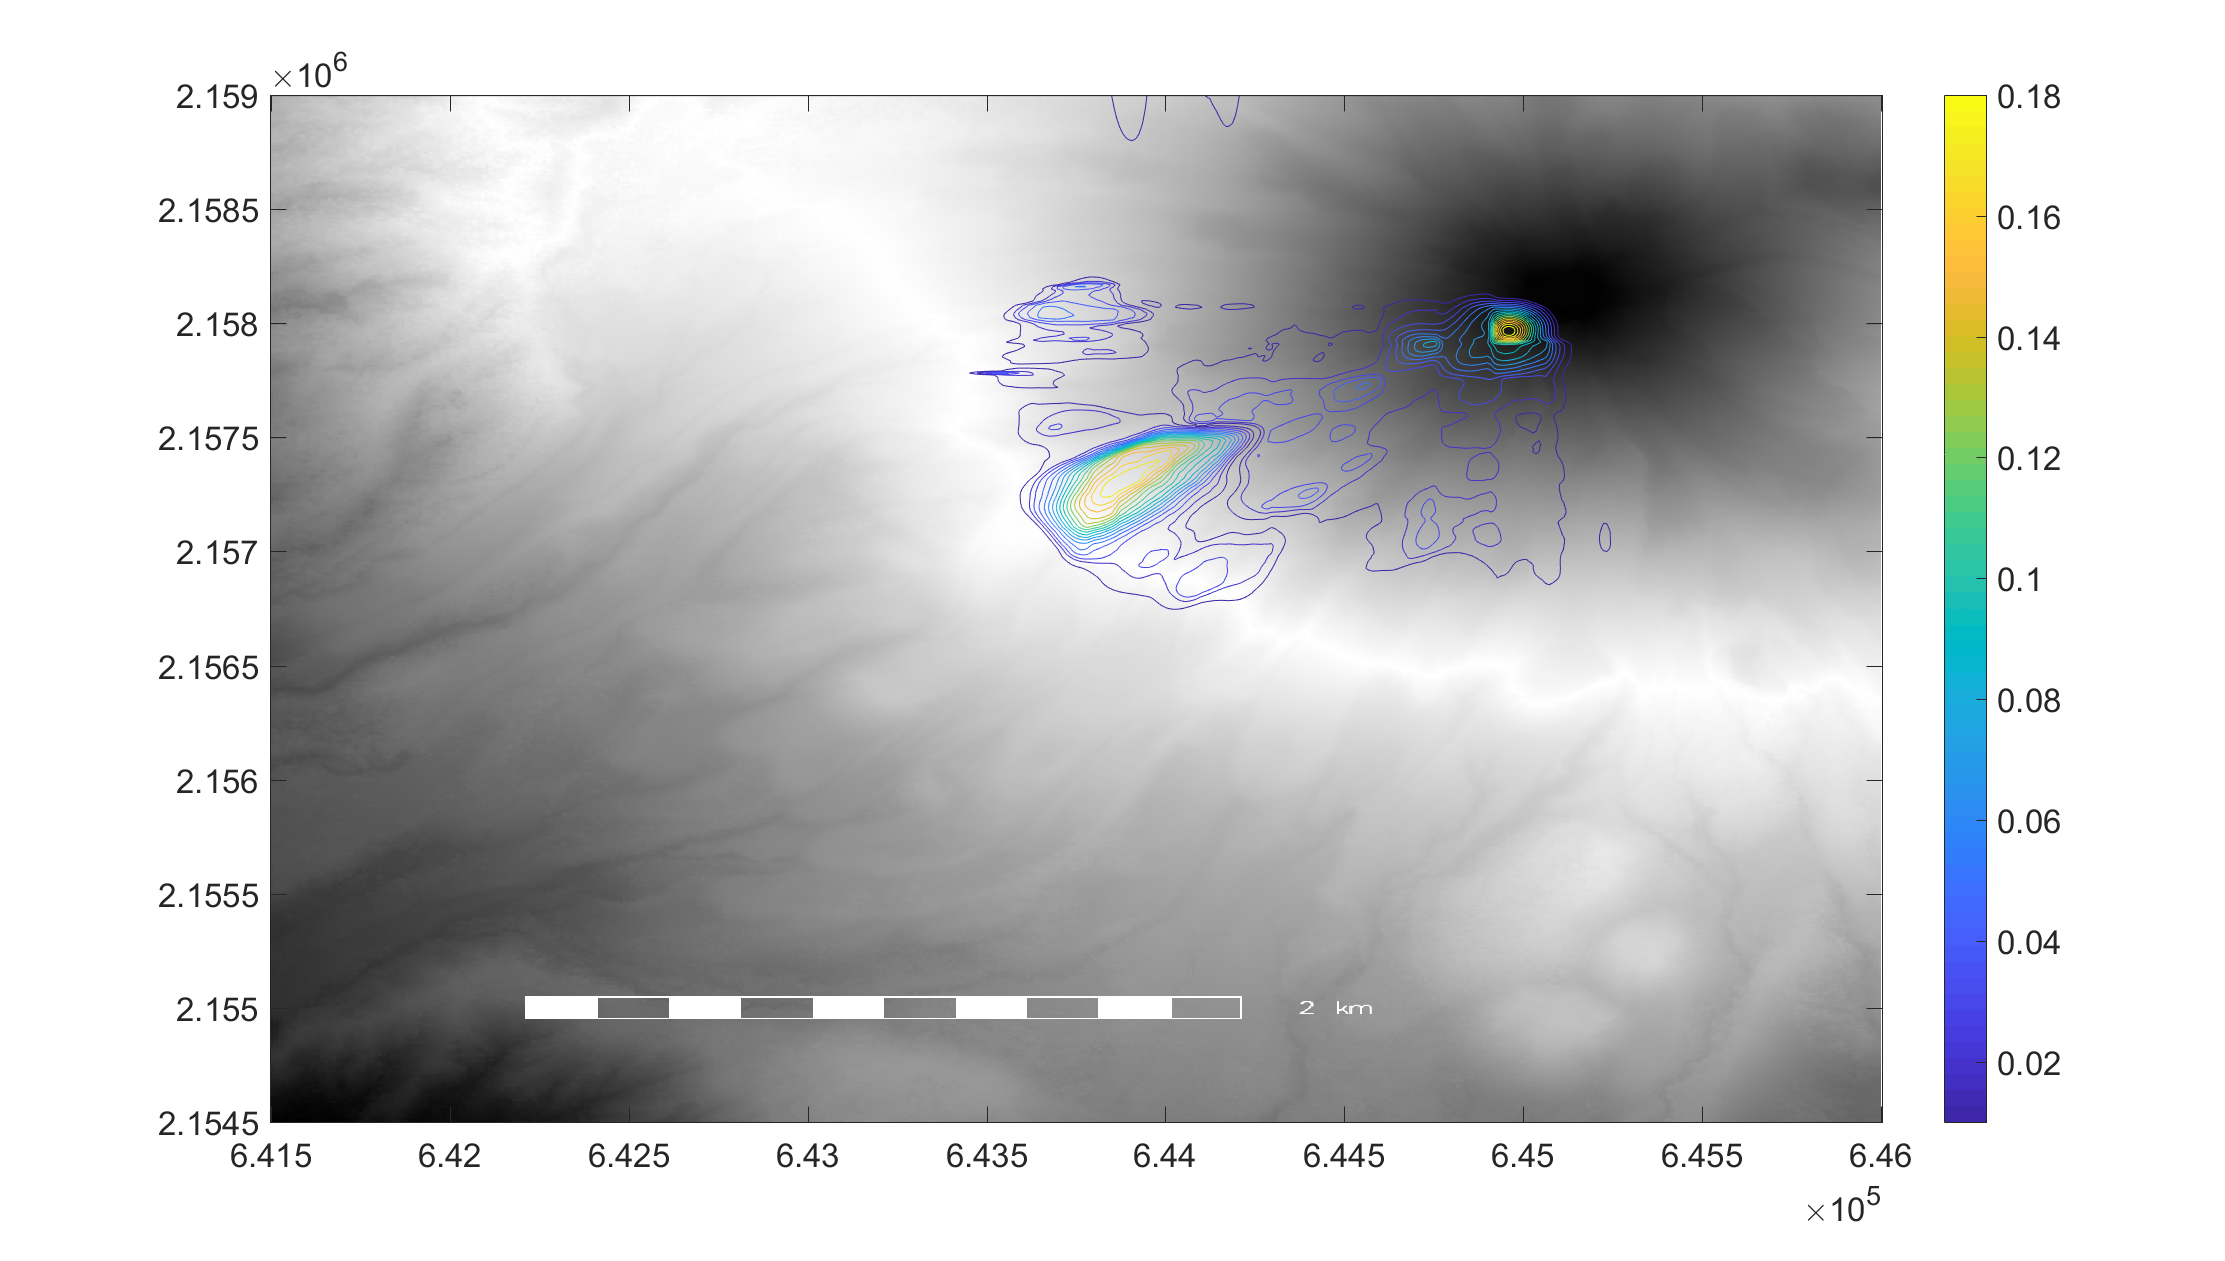
\includegraphics[width=\textwidth]{dem_figs/fig37}
\caption{at Time = 37s}
\end{subfigure}
\caption{Mean Pile height at different time instance}
\label{fig:colima_error}
\end{figure}

\section{Summary}

This chapter outlines the methodology in identifying sub-regions that contribute independently in parallel to the overall hazard map resulting from the geophysical mass flow simulation. The independent regions bears regional overlap that can be quantified using the suitable clustering method. Titan2D provides a robust platform to integrate with the proposed sampling scheme for generation of the PHMs. The outlined framework is able to achieve the target of generating sampling space in parallel as compared to any other sampling scheme for the same level accuracy. Computation of moments from the results of the CFD simulations can also be performed faster compared to traditional methods. It is shown that the applicability of SCS detection is universal in terms of sampling scheme. In other words SCS-based UQ approach can be integrated with any given sampling scheme. Some possible avenues for future works is discussed next.

In contrast to polynomial or exponential growth in standard cubature-based methods~\cite{stroud1971approximate}, the SCS-based method can produce a linear growth in number of collocation points with increase in the size of the problem. Thus, producing PHMs by integrating SCS-based UQ with cubature-based methods can be a scope of future work.

Even with the advantage of faster computation with the sampling scheme, formulation of the adjacency matrix can still be a non-trivial due to the size of the DEM. The current clustering paradigm takes advantage of asymptotic convergence of the cluster structure with increase in the resolution of the discretization. The adjacency formulation relies on vectorization and application of standard clustering techniques. The framework can be extended by taking the fourth order tensor adjacency followed by application of tensor-based overlapping community detection methods~\cite{benson2015tensor,shashua2005non,huang2013fast}.  

The SCS-based method has been useful for not only faster UQ but also in breaking the overall stochastic problem into subproblems. To incorporate the idea of subproblem decomposition into the PHM computation problem, one has to carefully define the boundary conditions in the identified subproblem, such that solving them in parallel bears a meaningful physical interpretation with respect to the full model. 